\documentclass[10pt,twocolumn]{wlscirep}
\usepackage[utf8]{inputenc}
\usepackage[T1]{fontenc}
\usepackage{tikz}
\usepackage{xcolor}
\usetikzlibrary{shapes.misc}
\newenvironment{Figure}
  {\par\medskip\noindent\minipage{\linewidth}}
  {\endminipage\par\medskip}

% Set left and right margins
\setlength{\rightmargin}{0.25in}
\setlength{\leftmargin}{0.25in}

\title{Can ENSO predict dengue outbreaks? A causal-based analysis on the role of climate patterns in \textit{Aedes}-borne disease transmission}

\author[1, 2*]{Javier Corvillo}
\author[2*]{Verónica Torralba}
\author[2]{Diego Campos}
\author[3]{Ana Riviére-Cinnamond}
\author[4]{Ángel G. Muñoz}

\affil[1]{Complutense University of Madrid, Department of Earth Science and Astrophysics, Madrid, 28040, Spain}
\affil[2]{Barcelona Supercomputing Center, Earth Sciences Department, 08034, Spain}
\affil[3]{Pan-American Health Organization, Communicable Diseases and Health Analysis, Panama City, 0843-03441, Panama}
\affil[4]{International Centre for Theoretical Physics, Trieste, 34151, Italy}
\affil[*]{javier.corvillo@bsc.es / veronica.torralba@bsc.es / angel.g.munoz@bsc.es}


\begin{abstract}
  \textbf{Background}: Vector-borne diseases transmitted by \textit{Aedes} mosquitoes such as dengue, Zika, and chikungunya, pose significant public health challenges worldwide in the wake of human-driven climate change. However, while their transmission is known to be susceptible to some climate variables like temperature, rainfall or humidity, the overall role of climate patterns on the emergence of these diseases is not so well understood.
  \\
  \\
\textbf{Methods}: Using data from a number of sources, we explore and analyse the response of \textit{Aedes}-borne disease transmission to climate patterns. Our analysis is composed of three different studies: 1) a timescale decomposition of disease transmissibility values, thereby guiding officials to understand the behaviour of outbreaks for budget and resource allocation; 2) a correlation analysis between transmissibility values and different seasonal climate variability modes, such as El Niño Southern Oscillation, in order to check for the influence of natural climate patterns onto \textit{Aedes}-borne outbreaks; and 3) a causality analysis to solidify findings obtained through correlation, identifying the most relevant predictors for \textit{Aedes}-borne diseases.
\\
\\
\textbf{Results}: Long-term, man-made climate change is shown to have a significant impact on the environmental suitability for \textit{Aedes}-borne diseases in the tropics, where El Niño Southern Oscillation and the Indian Ocean Basin are key climate patterns conditioning disease emergence. Temperate regions are shown to be more susceptible to seasonal climate variability, where multiscale climate patterns, through teleconnections and compound interactions, can influence transmission dynamics.
\\
\\
\textbf{Conclusions}: Disease transmission of \textit{Aedes}-borne diseases is shown to be susceptible to multiple factors, including long-term climate change and seasonal variability. The results of this study highlight the multi-faceted role of climate patterns in disease emergence, and their potential applicability in the development of early warning systems for \textit{Aedes}-borne disease outbreaks. Future research should focus on integrating these findings into an actionable \textit{Aedes}-borne seasonal prediction system using climate patterns as predictors, which can ultimately better inform public health strategies to manage dengue outbreaks.
\\
\\
\textbf{Keywords}: Public Health, Vector-borne Diseases, Epidemiology, Climate Change, Climate Services, Environmental Sciences
\end{abstract}
\twocolumn
\begin{document}

\flushbottom
\maketitle

\section*{Multilingual abstracts} \label{sec-abstract}

Please consult the \hyperref[sec-additional-files]{Additional files} section for abstract translations into the other five official languages of the United Nations (Arabic, Chinese, French, Russian and Spanish).

\section{Background} \label{sec-background}

\subsection{The emergence of vector-borne diseases in the context of climate change} \label{sec-background-vector-borne-diseases}

Disease stability and transmissibility under changing climate conditions has long been a topic of interest and research in the fields of epidemiology and virology. Many viral, bacterial, and parasitic diseases have been shown to be reactive to changes in environmental conditions across different regions and timescales \cite{thomson_2008, malloy_2019}. This is particularly true for previously pandemic diseases that have become endemic once proper disease control mechanisms are implemented by public health officials \cite{li_2019} . Prevalent respiratory viruses, such as H1N1 influenza or the novel SARS-CoV-2 virus, have been shown to reduce their dependency on human spread once losing their pandemic status, adopting defined climate-dependent seasonal patterns and becoming more prominent in temperate climates during the winter season \cite{shaman_2011, romerostarke_2021}.
\\
\\
For vector-borne diseases (VBDs), while many known socio-economic factors shape up the expanse of pathogens\cite{lippi_2018, ibarra_2013, stewart-ibarra_2014}, the relationship between climate and disease transmissibility is even more intertwined. Carriers such as arthropods, snails and slugs thrive under specific climate-dependent thresholds and conditions, and in the context of anthropogenic climate change, the effects of global warming and changing precipitation patterns have been shown to affect the overall spatial distribution of these vectors\cite{lowe_2018, messina_2016}.
\\
\\
Mosquitoes of the \textit{Aedes} genus, such as \textit{Aedes albopictus} and \textit{Aedes aegypti}, are of particular interest and importance in medium and low income countries \cite{campbell-lendrum_2015}. As the main carriers of diseases like dengue (DENV), chikungunya (CHIKV), and Zika (ZIKV), they pose a significant public health threat, traditionally in tropical and subtropical regions\cite{OMS_2020}. In the Americas, for instance, DENV impacts account for over 2 million disability adjusted life years worldwide \cite{yang_2021}, and a low estimated annual cost of about US\$2.1 billion \cite{shepard_2011}.
\\
\\
However, the effects of climate change are causing \textit{Aedes}-related diseases not only to emerge in new, previously unaffected regions, but also to increase their spread in areas where they were previously endemic\cite{quam_2015}. Along with compound changes in urbanization\cite{lee_2021a} and population growth\cite{struchiner_2015}, climate change is posited to be a major driver of increased DENV incidence in temperate climates\cite{kraemer_2015}, with the recent establishment of epidemic activity in parts of North America\cite{franklinos_2019}, Southeast Asia\cite{ooi_2009}, and detection of local transmission in southern European countries along the Mediterranean Basin\cite{ECDC_2024}. Equatorial tropical and subtropical zones like the Sub-Saharan Africa and northern South America have also been subject to higher incidence over the past 40 years\cite{nakase_2024}. While the current yearly incidence of DENV amounts to an average of 400 million cases per year\cite{pourzangiabadi_2025}, it is believed that the effects of climate change may put an additional 2.5 billion people at risk of DENV if \textit{Aedes} vectors were to be present in every region where the climate is suitable for their development\cite{nakase_2024}.


\subsection{Known drivers on \textit{Aedes}-borne disease transmission dynamics and their impact} \label{sec-background-aedes-borne-diseases}

The present available scientific literature highlights a profound influence of the environmental conditions over \textit{Aedes} mosquito proliferation, with temperature and precipitation being the two known primary climate drivers of \textit{Aedes}-borne disease transmission due to their impact on both vector and pathogen biology alike.
\\
\\
Many vector physiological processes (e.g., biting frequency, reproduction rates) as well as pathogen characteristics (e.g., extrinsic incubation duration) are conditioned by temperature, increasing until certain temperature thresholds are reached\cite{mordecai_2019}. In a similar manner, rainfall promotes the availability of mosquito breeding sites up until a critical point, in which excessive rainfall may flood or wash out the mosquito larvae away\cite{paaijmans_2007}. In conjunction, the combined effects of temperature and rainfall modulate the length of the \textit{Aedes}-borne transmission season of DENV, CHIKV and ZIKV in temperate areas and affected hotspots, with higher incidence particularly in urban areas of the Western Pacific and the Eastern Mediterranean regions\cite{colon-gonzalez_2021}.
\\
\\
Aside from these climate variables, humidity is also another probable factor in the proliferation of \textit{Aedes} mosquito breeding sites, though proper characterization and relationships with disease transmission remains a current object of study. Evidence suggests that elevated humidity levels could play a role in reducing incubation periods and blood-feeding cycle duration in \textit{Aedes} mosquitoes\cite{descloux_2012}.

\subsection{Climate patterns as an aggregate of unknown transmissibility drivers} \label{sec-climate-patterns}

While the aforementioned macro climatic factors have been widely used in \textit{Aedes}-borne disease research and modelling\cite{caminade_2017, liu-helmersson_2014, mordecai_2017, wesolowski_2015}, it is widely acknowledged that these are not enough to fully explain the climate component of \textit{Aedes}-borne disease transmissibility, and that more explanatory variables may aid in building more refined and actionable DENV monitoring and prediction systems\cite{erraguntla_2021, lee_2017, yavarinejad_2021, sriklin_2021}. Moreover, temperature and rainfall my also affect other possible small-scale climate modulators like soil moisture or vegetation growth, which in turn may affect the availability of breeding sites for \textit{Aedes} mosquitoes. Additionally, analysis of high resolution satellite imagery has suggested that land cover change, through deforestation, as well as stagnant water bodies, may also promote the proliferation of \textit{Aedes} breeding sites\cite{ali_2025}.
\\
\\
From a pragmatic perspective, understanding the contribution of each of these additional climate variables, each operating in different spatial and temporal scales, can be a challenging undertaking. Many of these variables lack comprehensive long-term observational records, particularly in tropical and southern regions where \textit{Aedes} diseases are most prevalent\cite{shaw_2024, senroy_2018}. Computational constraints may also arise when attempting to model multiple interacting variables simultaneously which, along with the sheer number of potential variables, makes it difficult to determine which combinations are most relevant for disease prediction without extensive resources. To add to this complexity, the effects of these variables may not be immediately apparent, as variables like soil moisture, for instance, do depend on many sub-processes as well\cite{peng_2023}.
\\
\\
It is for this reason why climate patterns, in this context, may serve a better role in mapping out the underlying climate processes behind \textit{Aedes}-borne disease transmission. Climate patterns are large-scale recurring ocean or atmospheric phenomena that can influence weather and climate conditions over different timescales (subseasonal, seasonal, inter-annual, decadal, etc.). They are often characterized by their periodicity, identified through their defined climate variability indices, and their effects ripple through the climate system, affecting temperature, precipitation, and other climate variables across different regions through teleconnections\cite{lubbecke_2018}.
\\
\\
As such, climate patterns may serve as aggregators of both large and small climate phenomena by linking various climatic oscillations to regional weather events and other environmental processes\cite{lee_2018}. Since they encapsulate broader climatic trends that affect local conditions, climate patterns seem preferable over everyday climate variables in the development of future climate-and-health \textit{Aedes} prediction systems\cite{easterbrook_2016, hallett_2004}. The analysis of seasonal patterns, such as the El Niño Southern Oscillation (ENSO), could provide insight as to how the complex interactions influence precipitation, temperature, and ultimately, \textit{Aedes}-disease transmission and emergence.

\subsection{The applicability of climate services in vector-borne disease prevention} \label{sec-climate-services}

Given the worldwide impacts of DENV, ZIKV and CHIKV and their expected potential to spread to unprepared regions, the need for effective \textit{Aedes}-borne disease control is more pressing than ever. To this end, many climate-and-health initiatives have been developed in recent years, with the aim of providing actionable information to public health officials and decision makers, such as the Tropical Disease Research initiative from the World Health Organization's (WHO)\cite{keating_2023, ramirez_2017}, as well as its Global Strategic Preparedness, Readiness and Response Plan, with \$55 million in funding from different stakeholders and public officials. Other examples include the mapping of environmental suitability for DENV, ZIKV and CHIKV\cite{munoz_2020a, guerra_2025}, or the development of integrated surveillance systems for \textit{Aedes} arboviruses\cite{leandro_2024}.
\\
\\
The development of early warning systems (EWS) for \textit{Aedes} vectors are also another area of focus in which climate information translates to more actionable health information\cite{ropelewski_1985}. While disease EWS can be based on clinical and empidemiological data alone, the integration of climate information at different timescales (subseasonal, seasonal, inter-annual, decadal) can improve the accuracy and skill of these systems while simultaneously extending the window over which changes in transmissibility can be detected\cite{thomson_2006, cox_2007}.
\\
\\
Here, we aim to characterise the behaviour and climatology of the climate-driven component of \textit{Aedes}-borne transmissibility, in order to understand its evolution over time in the context of climate change and how the different climate timescales may influence DENV outbreaks in different regions and seasons. Additionally, we aim to outline the role of climate patterns in the predictibility of \textit{Aedes}-borne disease emergence, in order to establish their relevance in operational vector-borne disease control programs and as predictors under a possible causal-based outbreak prediction system.

\section{Methods} \label{sec-methods}

We utilize a select number of datasets and methodologies to undertake three distinct analyses. By using global climate products that transform climate variables into the climate-driven component of \textit{Aedes}-borne transmissibility, we can explore its underlying mechanisms over affected and emerging areas at multiple timescales (seasonal, inter-annual, decadal, and long-term trends). We later employ a series of correlation and causality analyses for different climate patterns on \textit{Aedes}-disease emergence. By highlighting which climate patterns are dominant over the different areas and seasons, we can assess their impact on the transmissibility of \textit{Aedes}-borne diseases, therefore determining whether they may qualify as predictors for future DENV, ZIKV or CHIKV outbreaks.

\subsection{$R_0$ as a bridge between climate and health} \label{sec-methods-redefining-R0}

In recent years, at least three main mechanisms have been discussed to explain the seasonality of VBDs\cite{moriyama_2020}: the effects of the vector's behaviour (e.g. absence or presence in the area), human behaviour (e.g whether an infected host can transmit the disease by travelling), and the climate (whether the conditions are favourable for the vector to transmit the disease). These three mechanisms are usually encapsulated in the basic reproduction number, or $R_0$, which is a commonly used epidemiological metric that quantifies the transmissibility of VBDs, and is defined as the average number of secondary cases generated by a single infected individual in a susceptible population\cite{dietz_1993}.
\\
\\
However, while $R_0$ entangles vector, human, and climate behaviour, by only integrating the climate component of the disease transmission for the computation of $R_0$, then the resulting $R_0$ metric is more so interpreted as the role of environmental conditions in the spread of the disease. Thus, this definition of $R_0$, which we can understand as the diseases' environmental suitability, can be understood as a first approximation of the role of the climate in the dynamics of VBDs. This tweaked definition of $R_0$ is one of the operational outbreak indices commonly used by the WHO, along with several other decision-making institutes and health practitioners in disease control and prevention\cite{OMS_2017, chiew_2014}.


\subsection{The \textit{Aedes} Disease Environmental Suitability 2's monitoring system} \label{sec-methods-aedes2}

\begin{table*}[t]
  \centering
  \begin{tabular}{l|c|l|c}
    \textbf{Index Name}               & \multicolumn{1}{l|}{\textbf{Abbreviation}} & \textbf{Periodicity}          & \multicolumn{1}{l|}{\textbf{Pattern Type}} \\ \hline
    Atlantic 3 Index                  & ATL3                                       & Several months to a few years & Oceanic                                    \\
    Indian Ocean Basin Mode           & IOBM                                       & Several months to a few years & Oceanic                                    \\
    El Niño 3.4 Index                 & Niño 3.4                                   & Between 2-7 years             & Oceanic                                    \\
    North Pacific Meridional Mode     & NPMM                                       & Several months to a few years & Atmospheric                                \\
    South Atlantic Subtropical Dipole & SASD                                       & Several months to a few years & Oceanic                                    \\
    South Pacific Meridional Mode     & SPMM                                       & Several months to a few years & Atmospheric                                \\
    Tropical North Atlantic           & TNA                                        & Several months to a few years & Oceanic
  \end{tabular}%
  \caption{Summary of the climate variability indices used in the analysis used for the correlation and causality studies.}
  \label{tab:climate-variability-indices}
\end{table*}

The \textit{\underline{Ae}des} \underline{D}isease \underline{E}nvironmental \underline{S}uitability 2's (AeDES2) monitoring system\cite{guerra_2025} was used throughout this study in order to obtain the $R_0$ values for the analysis. Improving over its predecessor\cite{munoz_2020a}, AeDES2 is a climate-and-health service that provides real-time monitoring of the environmental suitability for \textit{Aedes}-borne diseases. The system uses known disease climate drivers like temperature and precipitation, and through its integration with ento-epidemiological models, as well as with calibration with recorded DENV cases, $R_0$ values are computed for different regions and seasons. The monitoring system is designed to be used by public health officials and researchers to assess the risk of disease outbreaks and to inform prevention and control strategies.
\subsection{Analysis 1: Multi-timescale climate decomposition of $R_0$} \label{sec-methods-1-analysis}

With the intent of isolating the signal of man-made climate change from the natural variability $R_0$ data, a timescale decomposition methodology was used to obtain the total variance across different timescales. This approach allows us to separate the complex $R_0$ signal into several time components, each providing insight into the climatological behaviour of \textit{Aedes}-borne disease transmission. This decomposition is particularly useful for health-officials in historically affected DENV hotspots, where understanding how different climate processes condition disease transmissibility is essential for the development of effective public health strategies, optimization of resource allocation, or implementation of targeted intervention strategies\cite{thomson_2018a, munoz_2016}.

\subsubsection{Data} \label{sec-methods-1-data}
The timescale decomposition analysis was undertaken using $R_0$ outputs from the AeDES2's monitoring system. The 1951-2024 monthly-mean period of AeDES2's $R_0$ values was selected for the analysis, for a total of 888 months or 295 full seasons. Considering that vector borne diseases are extending to previously unaffected areas due to the effects of man-made climate change, AeDES2's coverage has been increased since its inception to contain global outputs, allowing for a comprehensive analysis of the relationship between climate variability indices and $R_0$ in current \textit{Aedes} hotspots and emerging regions.

\subsubsection{Methodology} \label{sec-methods-1-methodology}

As $R_0$ doesn't follow a clearly defined probability distribution function, the timescale decomposition analysis filters a given $R_0$ time-series of any given grid-point by employing the non-parametric \underline{lo}cally \underline{e}stimated \underline{s}catterplot \underline{s}moothing technique (LOESS)\cite{jacoby_2000}. Sensitivity tests have been conducted in order to obtain the best LOESS smoothing parameter for the analysis, selecting the value that provides the lowest Generalized Correlated Cross-Validation ($GCV$) verification metric for the goodness of fit of the model\cite{craven_1978}. GCV was chosen amongst different metrics, as it provides a robust assessment of model generalizability by directly penalizing overfitting through its leave-one-out validation procedure\cite{marcotte_1995}.
\\
\\
Once the ideal LOESS smoothing parameter is found for the $R_0$ data, the $R_0$ time-series for each grid-point is separated into four components: a long-term trend signal (understood to be the trend caused by anthropogenic climate change), a seasonal signal (over-the-year change), a decadal signal (10-30 years), and lastly, a residual signal which contains other signals of the data (i.e., inter-annual and inter-decadal variability, among others). Variance maps for each of these four components capture the overall direction of the data over time, as well as the climatological variability of $R_0$ in any given grid-point.
\\
\\
After the variance maps are obtained, the trend of $R_0$ values is removed for the following correlation and causality analyses. While detrending through the assumption that $R_0$ changes linearly over time could be a valid approach, it fails to capture the temperature dependency of the data. In order to account for this intrinsic relationship of $R_0$ with temperature, a similar timescale decomposition analysis is performed on the detrended $R_0$ data, though instead of time as the independent variable, temperature data from the AeDES2's monitoring system datasets is used instead (monthly-mean temperature data consisting of the GHCN-CAMS project\cite{fan_2008}, the CPC Unified Global Temperature dataset\cite{xie_2007}, and the ERA5 and the ERA5Land reanalysis datasets\cite{chen_2008}). In this way, the obtained trend serves as a functional relationship between temperature and $R_0$: a temperature-based description of the $R_0$ signal, attributed to the warming of the planet\cite{greene_2011}.

\subsection{Analysis 2: Correlation studies between $R_0$ and climate variability indices} \label{sec-methods-2}
After analyzing the $R_0$ signal and its variability through timescale decomposition, we assess the impact of several climate variability indices on global $R_0$ values over the chosen 1951-2024 monthly-mean period.

\subsubsection{Data} \label{sec-methods-2-data}

Correlation studies are performed over global outputs, using the temperature-based detrended $R_0$ data as in the previous analysis over the different seasons. A total of 9 temperature-based climate variability indices have been used for the correlation analysis, which have been computed using the detrended temperature data utilized in the previous analysis. Their periodicity, as well as their main pattern type, are listed and summarized in Table \ref{tab:climate-variability-indices}.


\subsubsection{Methodology} \label{sec-methods-2-methodology}

The correlation analysis was performed using the Spearman partial correlation coefficient, which assesses how well an arbitrary monotonic function can describe the relationship between two variables\cite{spearman_1904}. For computation of statistical significance in correlation, the non-parametric Monte Carlo method was used\cite{new_2000}, with a p-value threshold of 0.05.


\subsection{Analysis 3: Causality studies between $R_0$ and climate variability indices. Outlining of predictors for disease outbreaks} \label{sec-methods-3}

Causal-based patterns can be identified after this analysis, which allow for a robust foundation for understanding of the underlying mechanisms between climate variability and $R_0$ patterns. These causality studies are performed over global outputs and over the different seasons. Along with results obtained through correlation, this causality analysis can be used to outline the most relevant predictors for disease outbreaks. These predictors, in turn, can be used for the refining and building of AeDES2's prediction system for improving the accuracy and skill of the ensemble forecasts compared to its predecessor.

\subsubsection{Data} \label{sec-methods-3-data}

The datasets that were used for the causality analysis are the same detrended datasets as those employed in Section \ref{sec-methods-2-data}.

\subsubsection{Methodology} \label{sec-methods-3-methodology}

Causality analyses between $R_0$ and climate variability indices were performed by using Liang-Kleeman's proposed methodology for computing information flow between two entities of a dynamical system, quantifying the amount of information that one time series (the climate variability indices) can provide about another time series ($R_0$ patterns)\cite{liang_2014}. Once the transfer entropy is computed, it is then normalized in order to account for the different scales of the two time series\cite{liang_2015}. Statistical significance is computed using Fisher's information matrix, with a p-value threshold of 0.05.

\section{Results}
\subsection{Analysis 1: Multi-timescale climate decomposition of $R_0$} \label{sec-results-1}

\begin{figure*}[!ht]
  \centering
  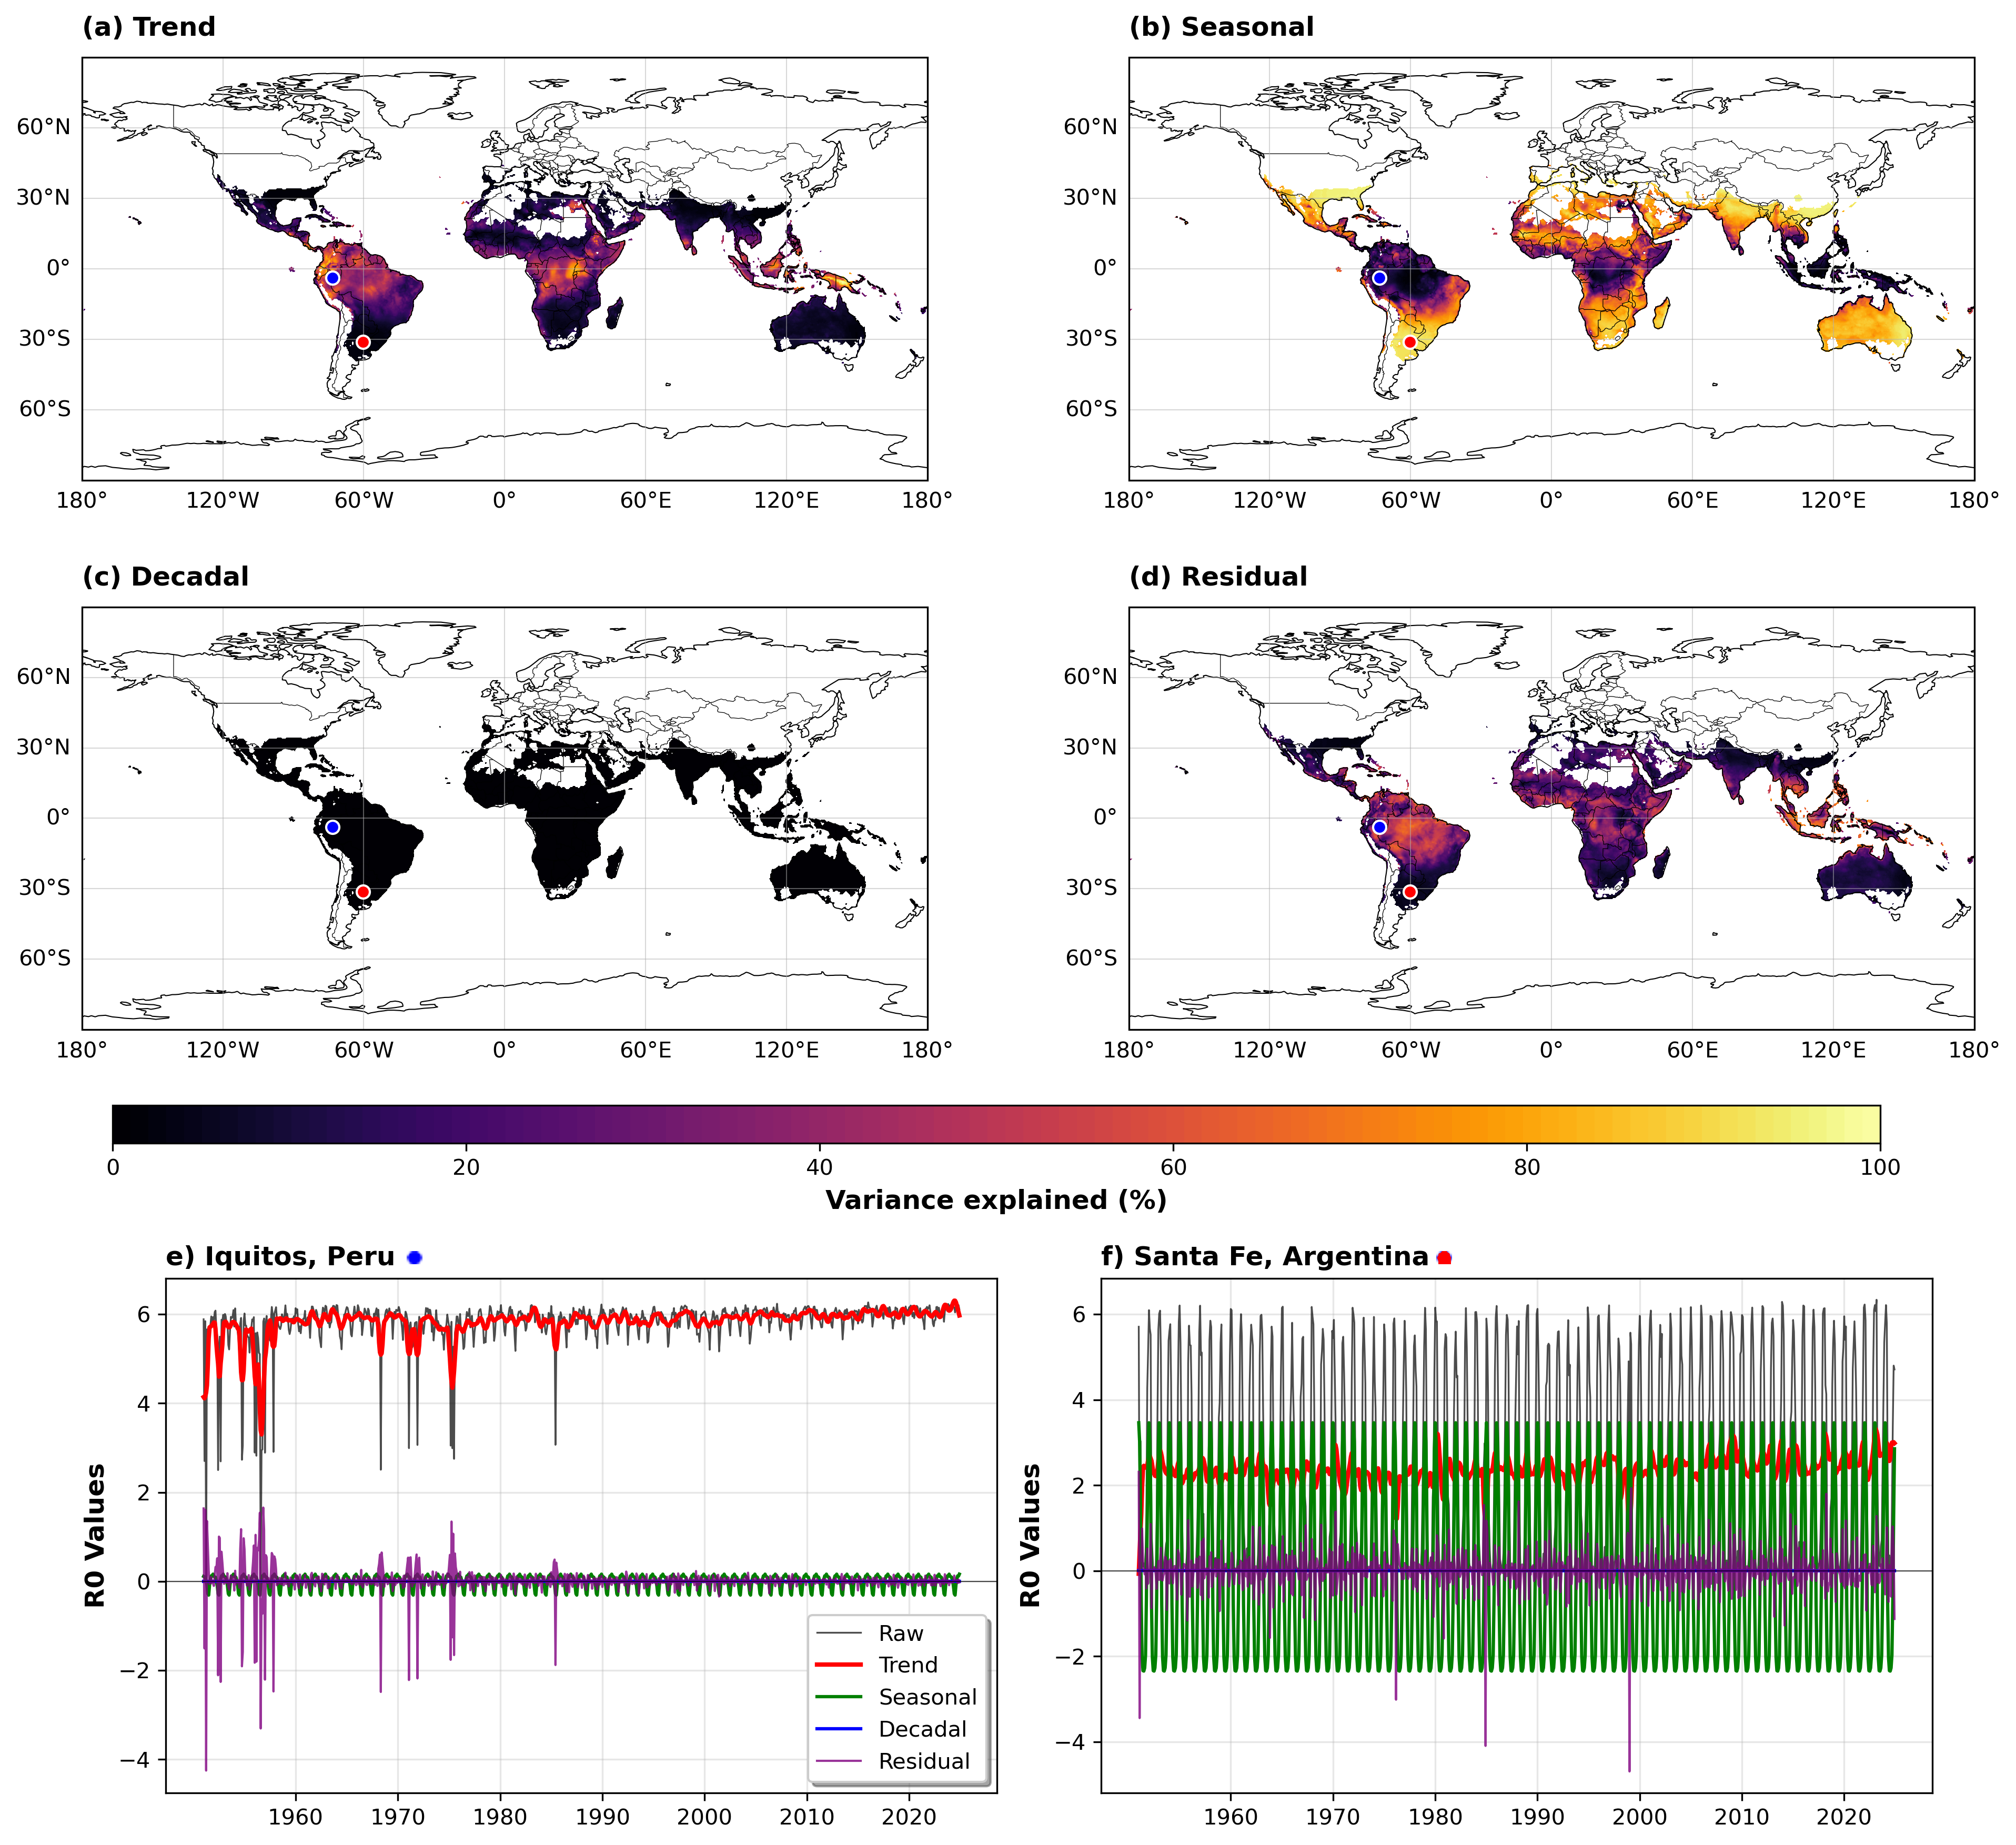
\includegraphics[width=\textwidth]{timescale_decomposition_combined_ps.png}
  \caption{\textbf{a)-d)} Global timescale decomposition maps for $R_0$ values for the monthly mean 1951-2024 period, different components. The time series for the cities of Iquitos, Peru (blue dot), and Santa Fe, Argentina (red dot), are shown as examples in \textbf{e)} and \textbf{f)} respectively.}
  \label{fig:global-timescale-decomposition}
\end{figure*}
\begin{figure*}[!ht]
  \centering
  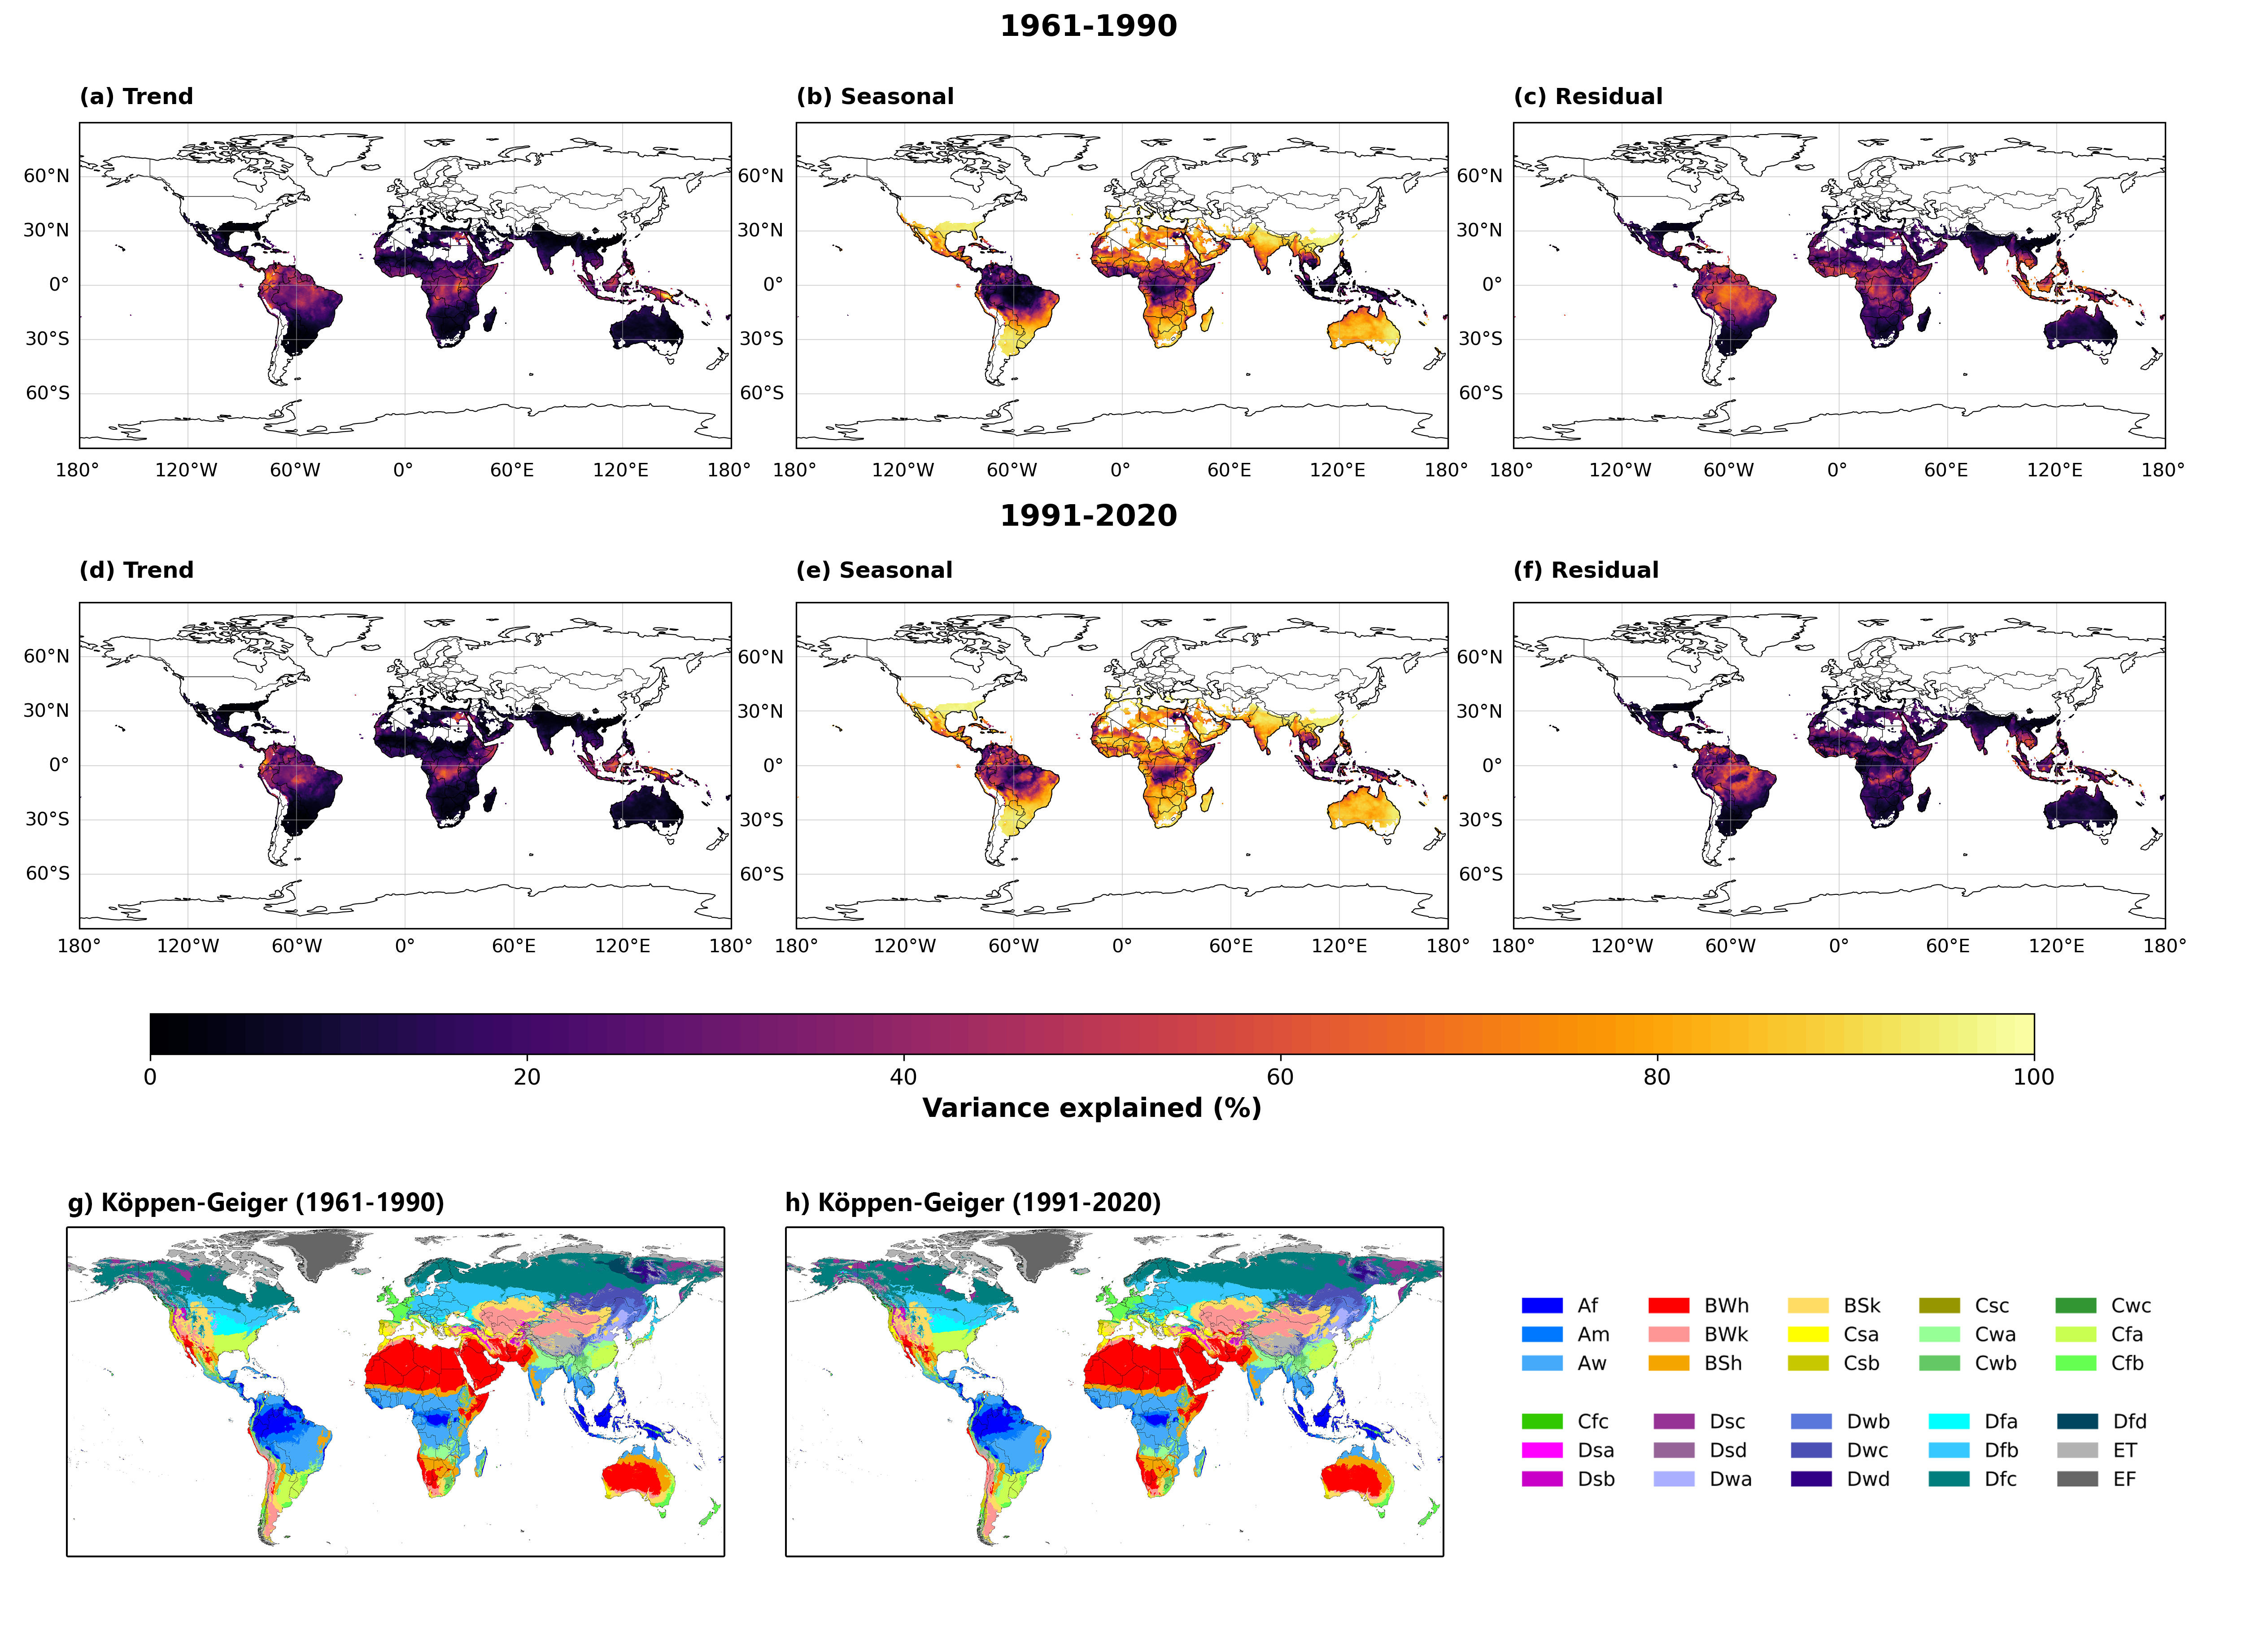
\includegraphics[width=\textwidth]{timescale_decomposition_climatology_comparison_ps.png}
  \caption{\textbf{a)-c)} Global timescale decomposition maps for $R_0$ values for the monthly mean 1961-1990 period, different components. Its associated Köppen-Geiger climate classification is shown in \textbf{g)}. \textbf{d)-f)} Global timescale decomposition maps for $R_0$ values for the monthly mean 1991-2020 period, different components. Its associated Köppen-Geiger climate classification is shown in \textbf{h)}. (Source for Köppen-Geiger climate classification maps: \cite{beck_2023})}
  \label{fig:global-timescale-decomposition-2}
\end{figure*}

The resulting timescale decomposition maps for $R_0$ global outputs for the whole time series can be found in Figure \ref{fig:global-timescale-decomposition}, along with the component time series for the cities of Iquitos, Peru, known to be a traditional hotspot of \textit{Aedes}-borne diseases, and Santa Fe, Argentina. The optimal span values of LOESS smoothing for the timescale decomposition methodology for this sample period was found to be 8 months for the $GCV$ verification metric. It is worth noting that, because the $R_0$ metric operates in certain temperature ranges, grid points with less than 6 months of data per year were excluded from the analysis, in order to prevent poor seasonal component estimation due to missing entire seasons.
\\
\\
Over the 74-year period, the long-term trends and residual components of $R_0$ (Figures \ref{fig:global-timescale-decomposition}a and \ref{fig:global-timescale-decomposition}d) show the highest variance contribution in tropical and subtropical regions, particularly across central Africa, parts of South America including the Amazon basin, and scattered areas in Southeast Asia and northern Australia (the sum of these components rounding between 40-80\%). These trend patterns suggest that long-term climate change, along with interannual climate variability, is driving systematic shifts in $R_0$ in these traditionally endemic regions, reflecting the complex interactions between temperature, humidity, and precipitation influencing vector populations and virus transmission. For these regions, there is no clearly defined transmission season over the year, as the seasonal signal of $R_0$ (Figure \ref{fig:global-timescale-decomposition}b and \ref{fig:global-timescale-decomposition}e) is rather poor. Instead, the climatology of $R_0$ in these regions, due to the high temperature and humidity values, adopts high $R_0$ values which remain constant throughout the year, independently of the season.
\\
\\
Though the decadal component (Figure \ref{fig:global-timescale-decomposition}c) shows a nigh negligible contribution across all regions of the globe (<5\%, Figure \ref{fig:global-timescale-decomposition}b), the seasonal variance shows a markedly different geographical distribution, with the highest contributions concentrated in regions with pronounced seasonal temperature variations (between 60-100\% variance explained). Notable hotspots include the northern edges of traditional DENV transmission zones in South America, parts of southern Africa, central Asia, and importantly, temperate regions that border current endemic areas. It is in these regions where the seasonal temperature fluctuations strongly condition the transmissibility season of $R_0$, reaching its peak around the summer months.
\\
\\
Indeed, Figure \ref{fig:global-timescale-decomposition}f highlights the effect of the seasonal component on the overall $R_0$ dynamics in these strong seasonal regions. While the trend component accounts for a significant portion of the variance, it is the seasonal component that can play a crucial role in defining whether a DENV outbreak can occur ($R_0$ > 1) or not ($R_0$ < 1).
\begin{figure*}[!ht]
  \centering
  \includegraphics[width=\textwidth]{correlation_seasonal_global_niño_34_ps.png}
  \caption{\textbf{a)-d)} Correlation values between $R_0$ and the Niño 3.4 index, for the 1951-2024 monthly mean period in all seasons. Dots represent statistically significant correlation values, at $p < 0.01$.}
  \label{fig:global-correlation-niño-34}
\end{figure*}
\\
\\
By dividing the full time series into two climatological subsets, the timescale decomposition methodology for each allows to see how the different components have evolved overtime. Two climatologies, corresponding to the 1961-1990 and 1991-2020 periods, can be found in Figure \ref{fig:global-timescale-decomposition-2}, along with their respective Köppen-Geiger climate classification maps\cite{beck_2023}. For both of these two periods, the GCV-optimal span value of LOESS smoothing is also 8 months, same as for the complete time series. The decadal component is not shown in this figure, as it remains negligible (<5\%) for both climatologies.
\\
\\
When examining the variance patterns in relation to the Köppen-Geiger classification, distinct climate zone signatures can become apparent on a first-approximation basis. Tropical climate zones (A-type climates in the Amazon basin, central Africa, and Southeast Asia) demonstrate characteristic patterns where trend and residual variance typically dominates. Alternatively, temperate and humid subtropical zones (C-type climates in southern Brazil, parts of East Asia, and the Mediterranean basin) show a more pronounced seasonal component. At a glance, it may seem that a study on the expansion of A and C type Köppen Geiger climates in the context of climate change may provide a useful framework for predicting the evolution of \textit{Aedes}-borne transmissibility, with each major climate type exhibiting distinct characteristics that condition the behavior of the $R_0$ signal.
\\
\\
However, this would be a naive approach, since the Köppen-Geiger classification is a static classification system that does not thoroughly reflect the dynamic nature of climate change\cite{triantafyllou_1994}. Indeed, the comparison between the two 30-year periods reveals notable shifts in how climate variability affects $R_0$ across different regions. In the 1961-1990 period, the trend component shows more concentrated high-variance zones, particularly in central Africa and tropical parts of South America. By the later 1991-2020 period however, these trend patterns have intensified in some regions while diminishing in others, highlighting that the impacts of systematic climate change on transmission potential, while shown to have become more pronounced over time, are not entirely straightforward.
\\
\\
Given the strong seasonality of $R_0$ in temperate regions through these timescale decomposition analyses, and given the different climate variables that \textit{Aedes}-borne transmissibility seems to relate to besides temperature, it is not unreasonable to expect $R_0$ values to be closely related to seasonal, temperature-driven climate patterns, be it in the form of correlation or causality. The following analyses aim to explore these relationships further, with the seasonal, temperature-driven climate variability indices previously listed in Table \ref{tab:climate-variability-indices}.

\subsection{Analysis 2: Correlation studies between $R_0$ and climate variability indices} \label{sec-results-2}

Spearman partial correlation outputs between $R_0$ and the Niño3.4 index for all seasons of the time series are shown in Figure \ref{fig:global-correlation-niño-34}. The most consistent positive correlations across seasons appear in the Amazon basin and northeastern South America, tropical A-type climate regions in the Köppen Geiger classification that correspond to areas of high trend and residual variance in the previous timescale analyses of section \ref{sec-results-1}. The austral summer and autumn seasons (figures \ref{fig:global-correlation-niño-34}a and \ref{fig:global-correlation-niño-34}b) show the highest positive correlation values in those regions, with Africa exhibiting more heterogeneous patterns with both positive and negative correlation zones in the austral autumn. It is during these months that we also observe notable emergence of negative correlations in parts of Southeast Asia, along with the appearance of positive correlations in some temperate transition areas as well.
\\
\begin{figure*}[!ht]
  \centering
  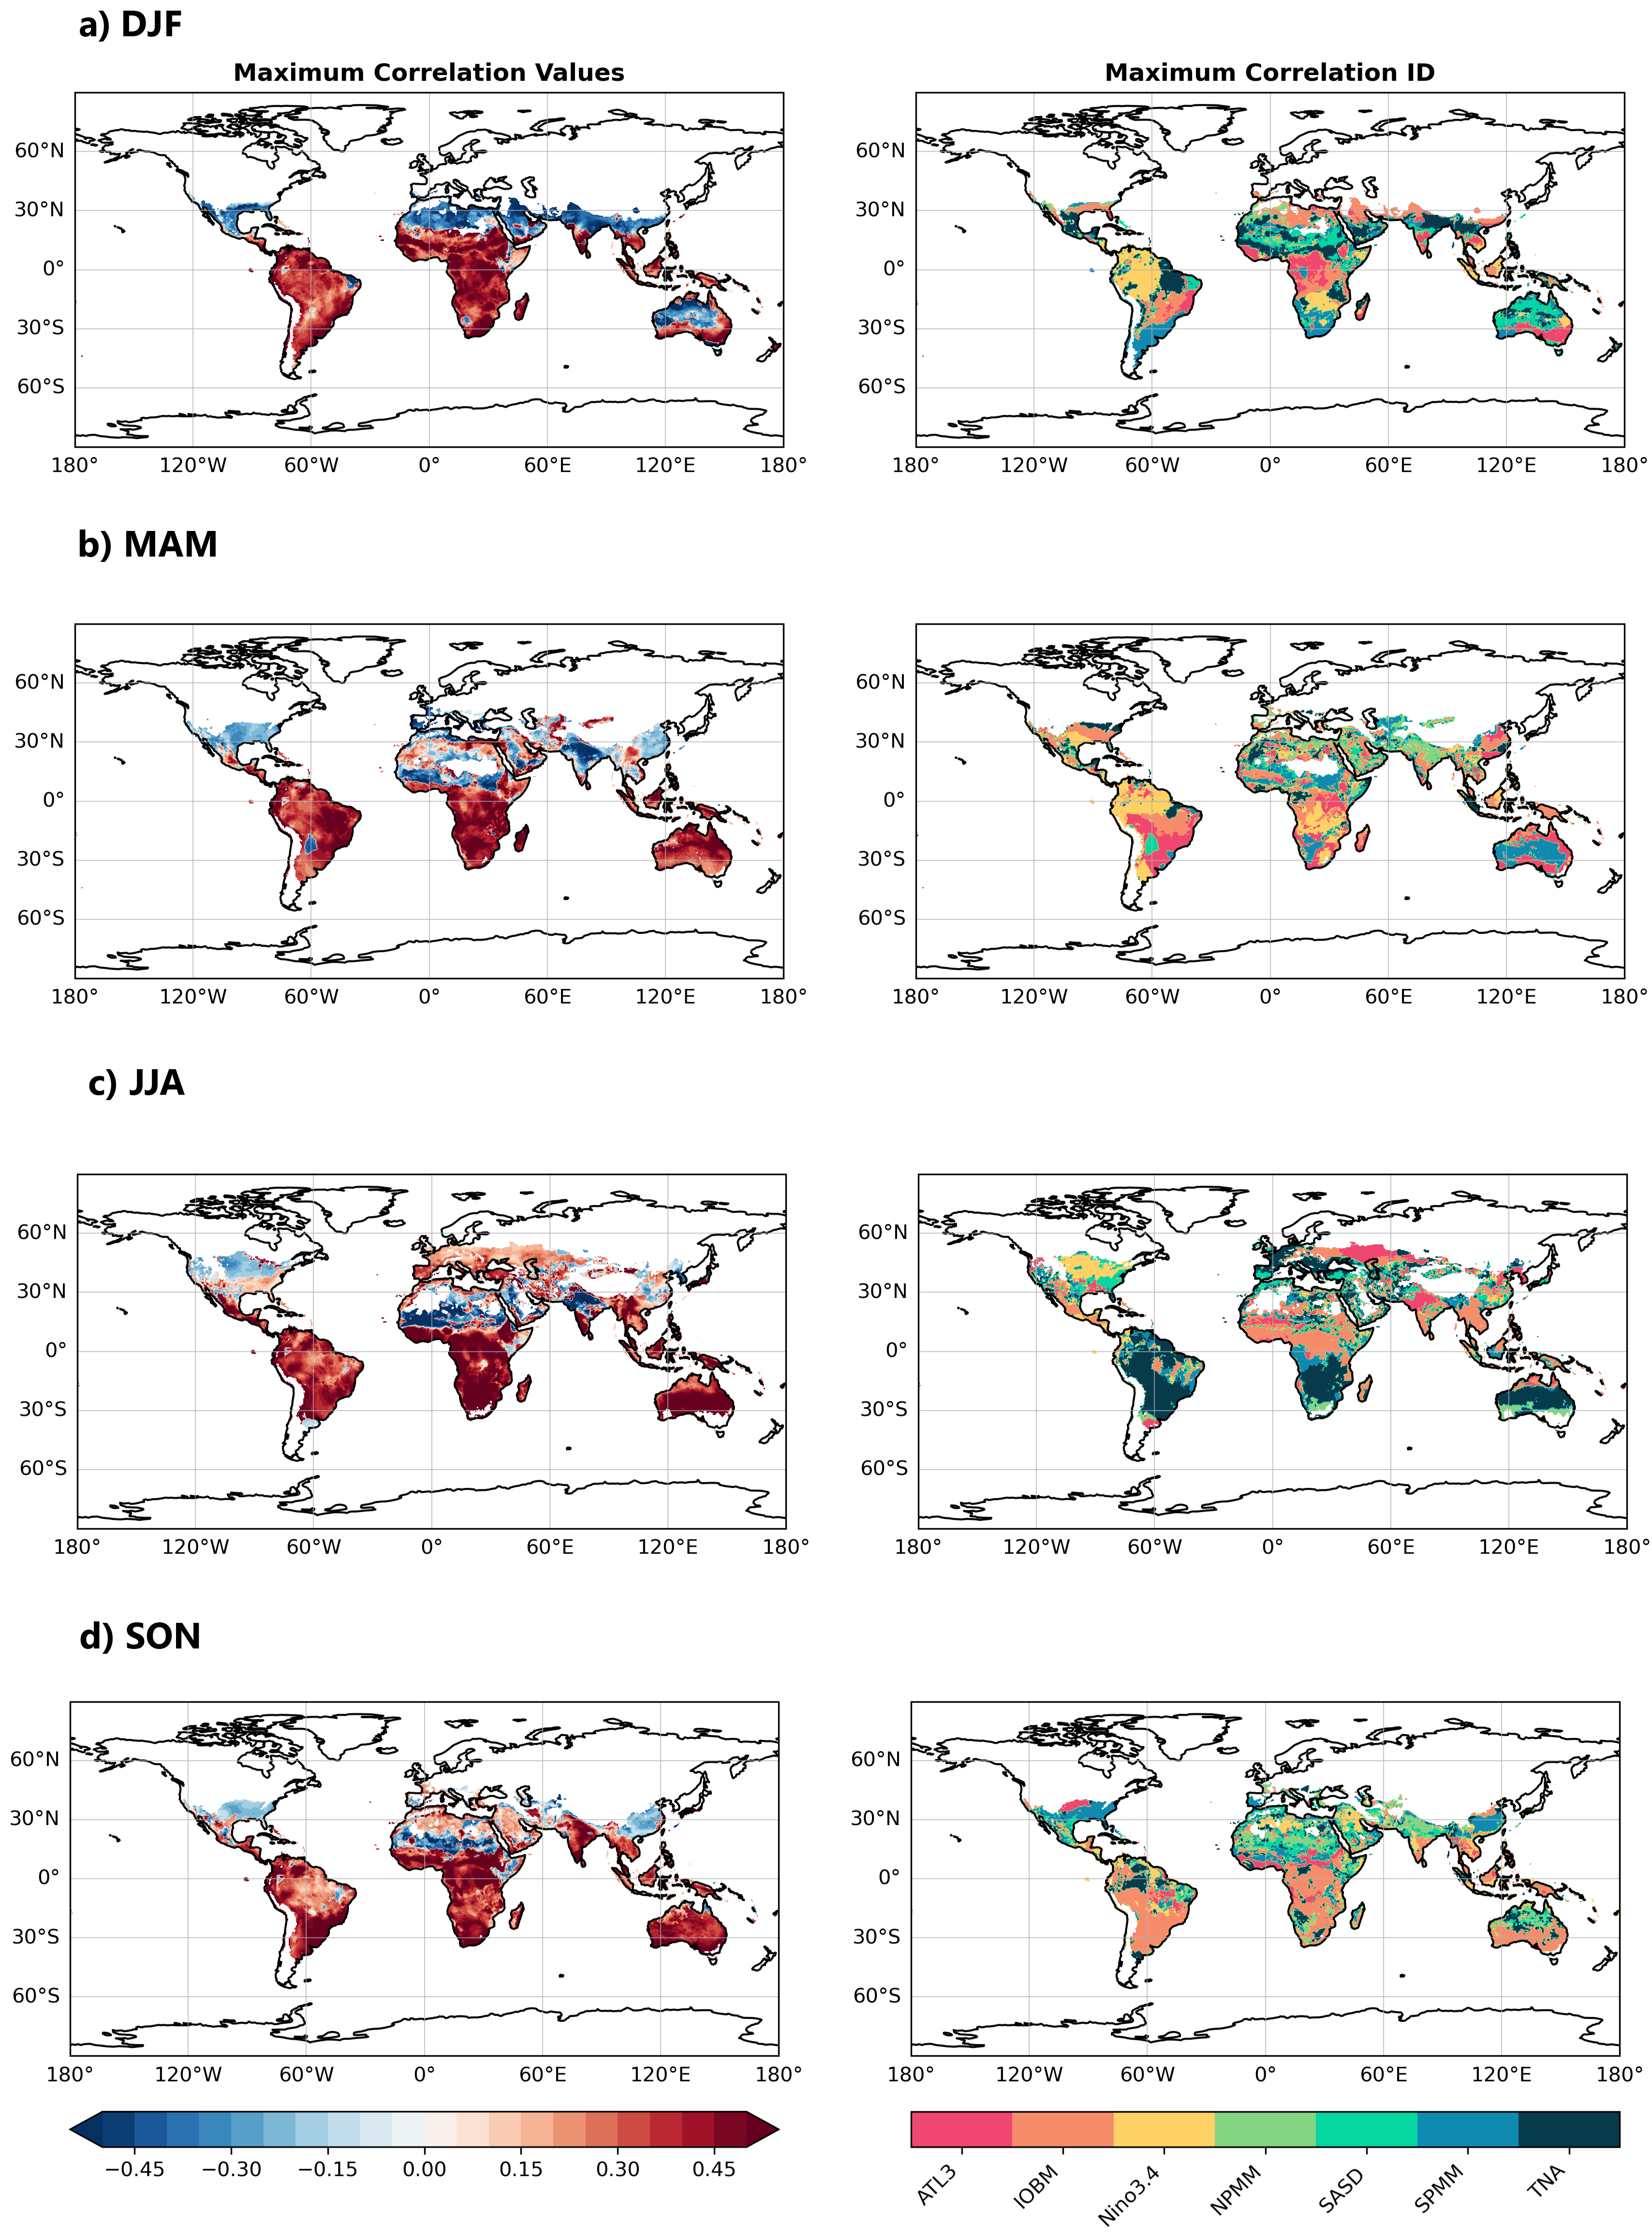
\includegraphics[width=0.9\textwidth]{correlation_final_global_ps.png}
  \caption{\textbf{a)-d)} For all seasons: Left, maximum statistically significant correlation values between $R_0$ and all indexes of Table \ref{tab:climate-variability-indices}, for the 1951-2024 monthly mean period ($p < 0.01$). Right, which climate index gives the maximum statistically significant correlation values.}
  \label{fig:global-correlation-final}
\end{figure*}

\begin{figure*}[!ht]
  \centering
  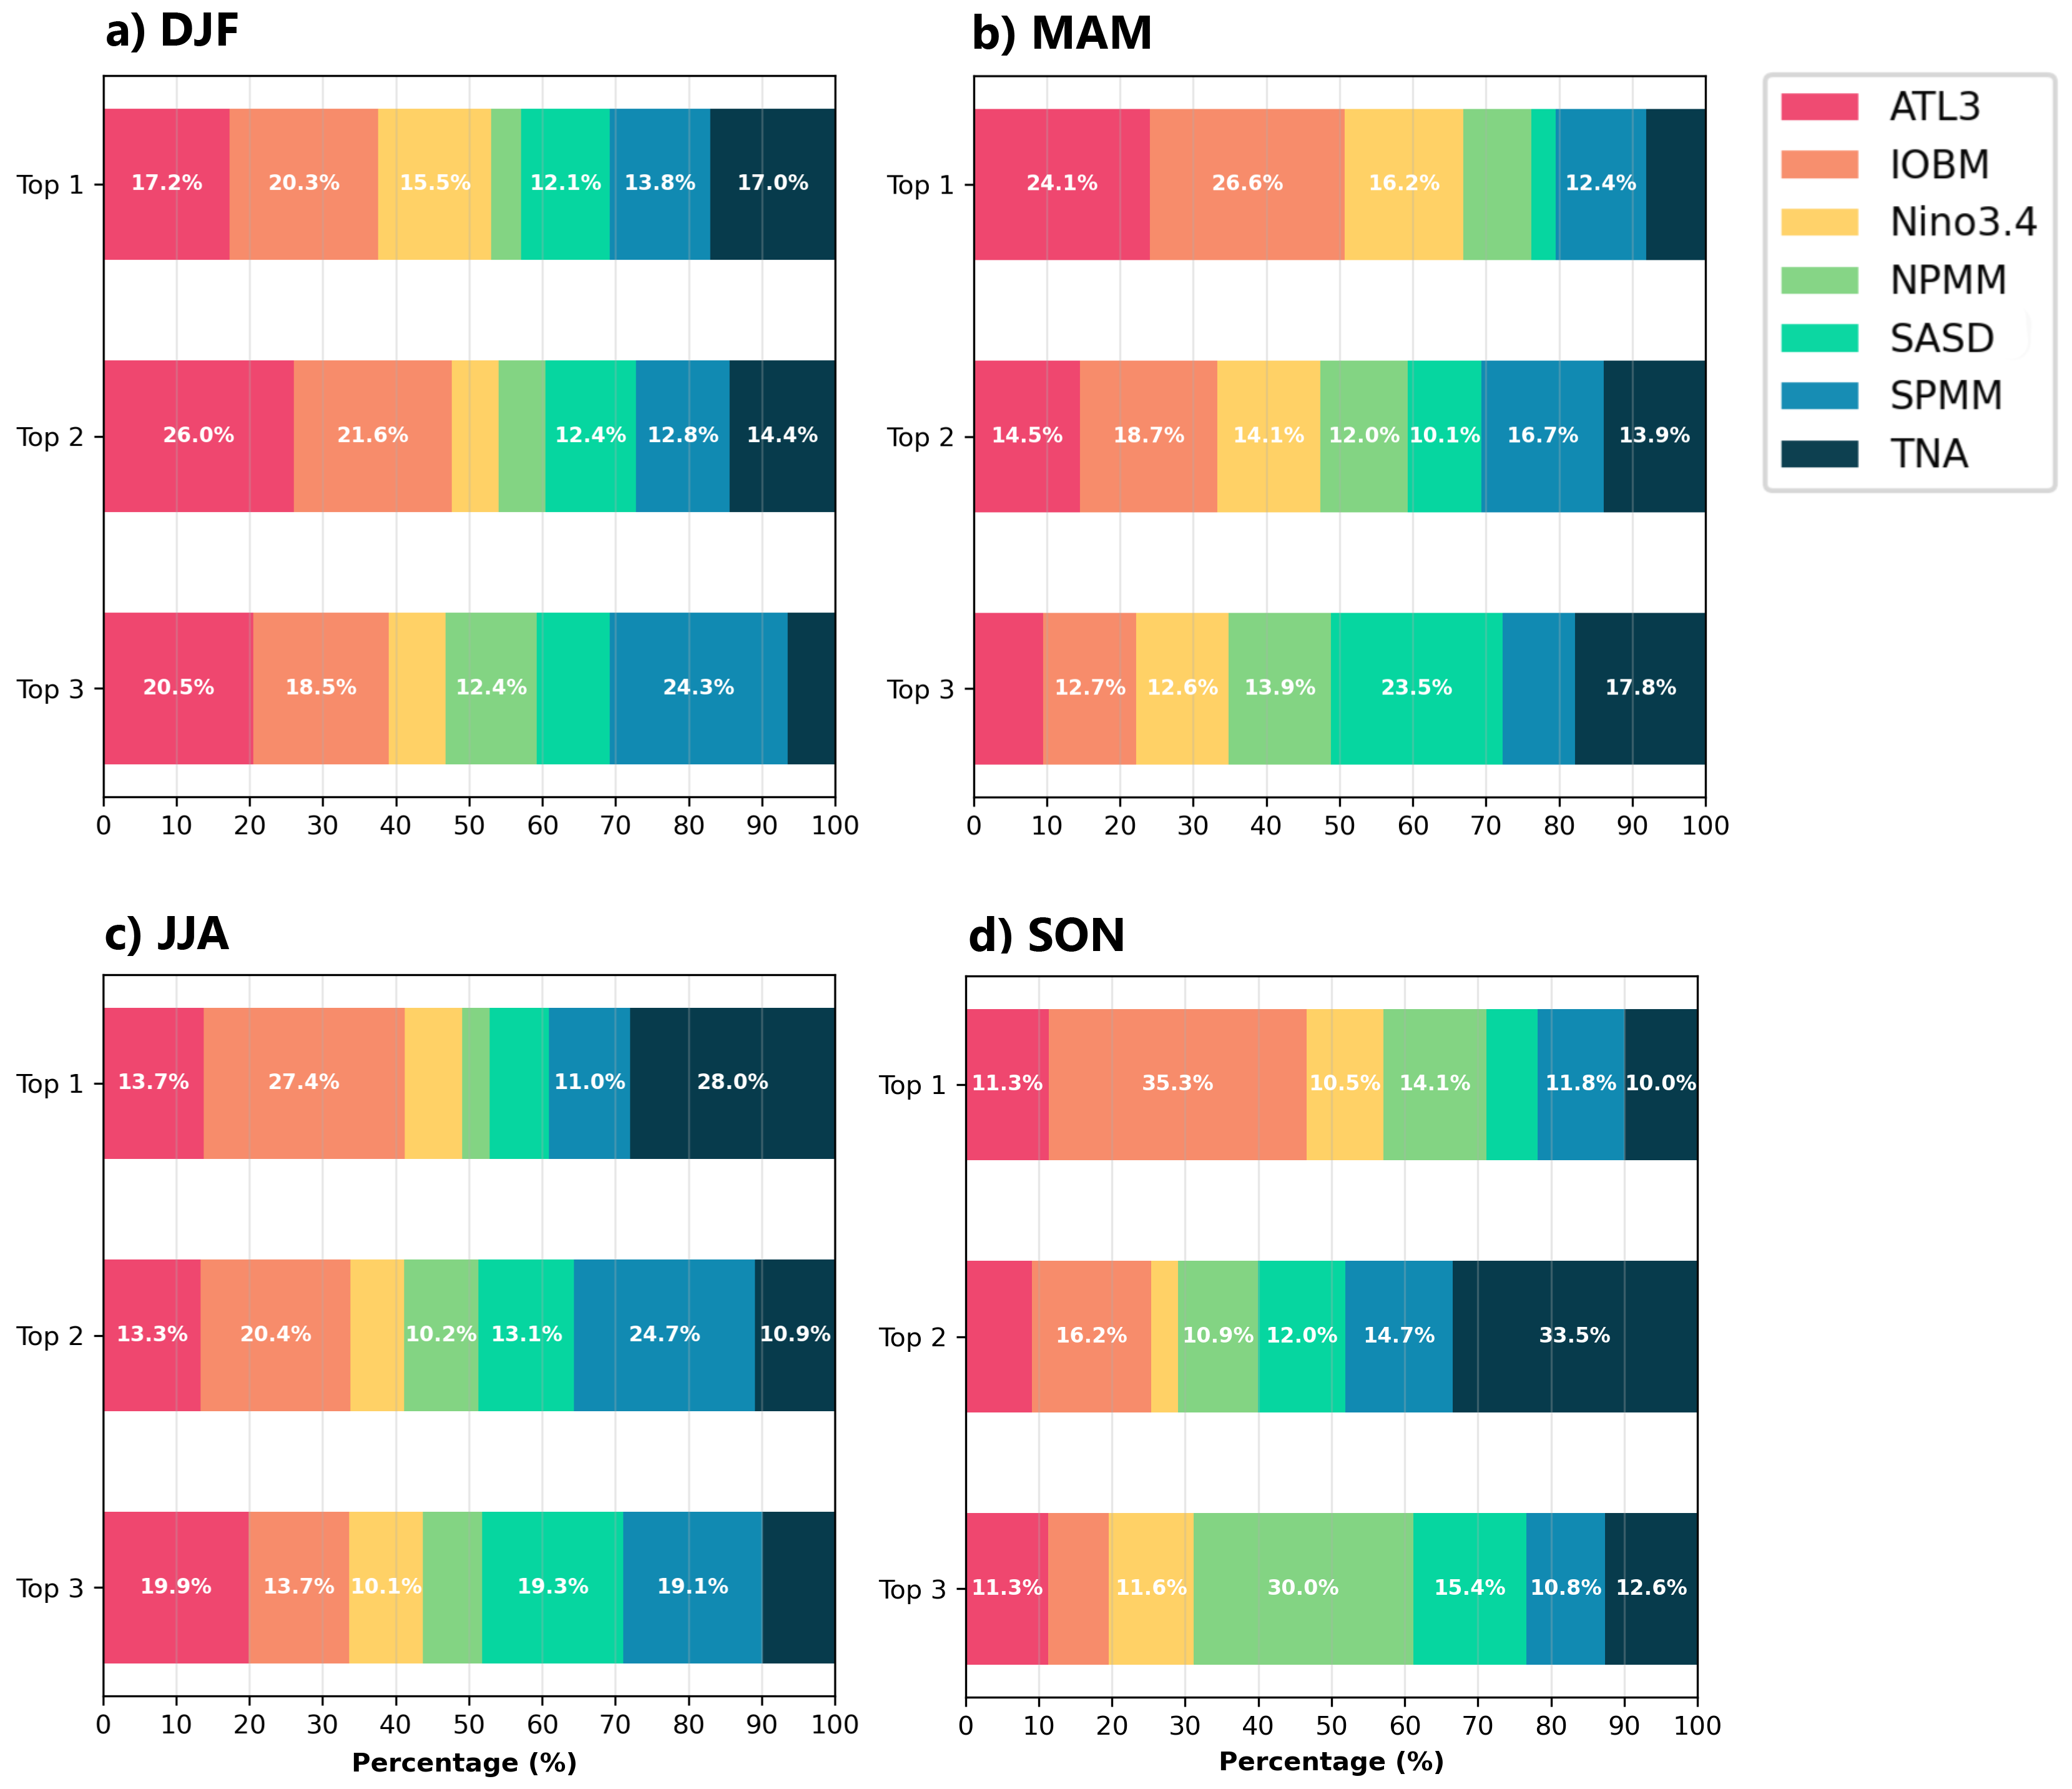
\includegraphics[width=0.75\textwidth]{correlation_barplots.png}
  \caption{\textbf{a)-d)} For all seasons: Percentage of grid points over which each index gives the highest, second or third highest statistically significant correlation values. Any contribution above 10\% is labeled in the barplots.}
  \label{fig:barplots-correlation}
\end{figure*}

\begin{figure*}[!ht]
  \centering
  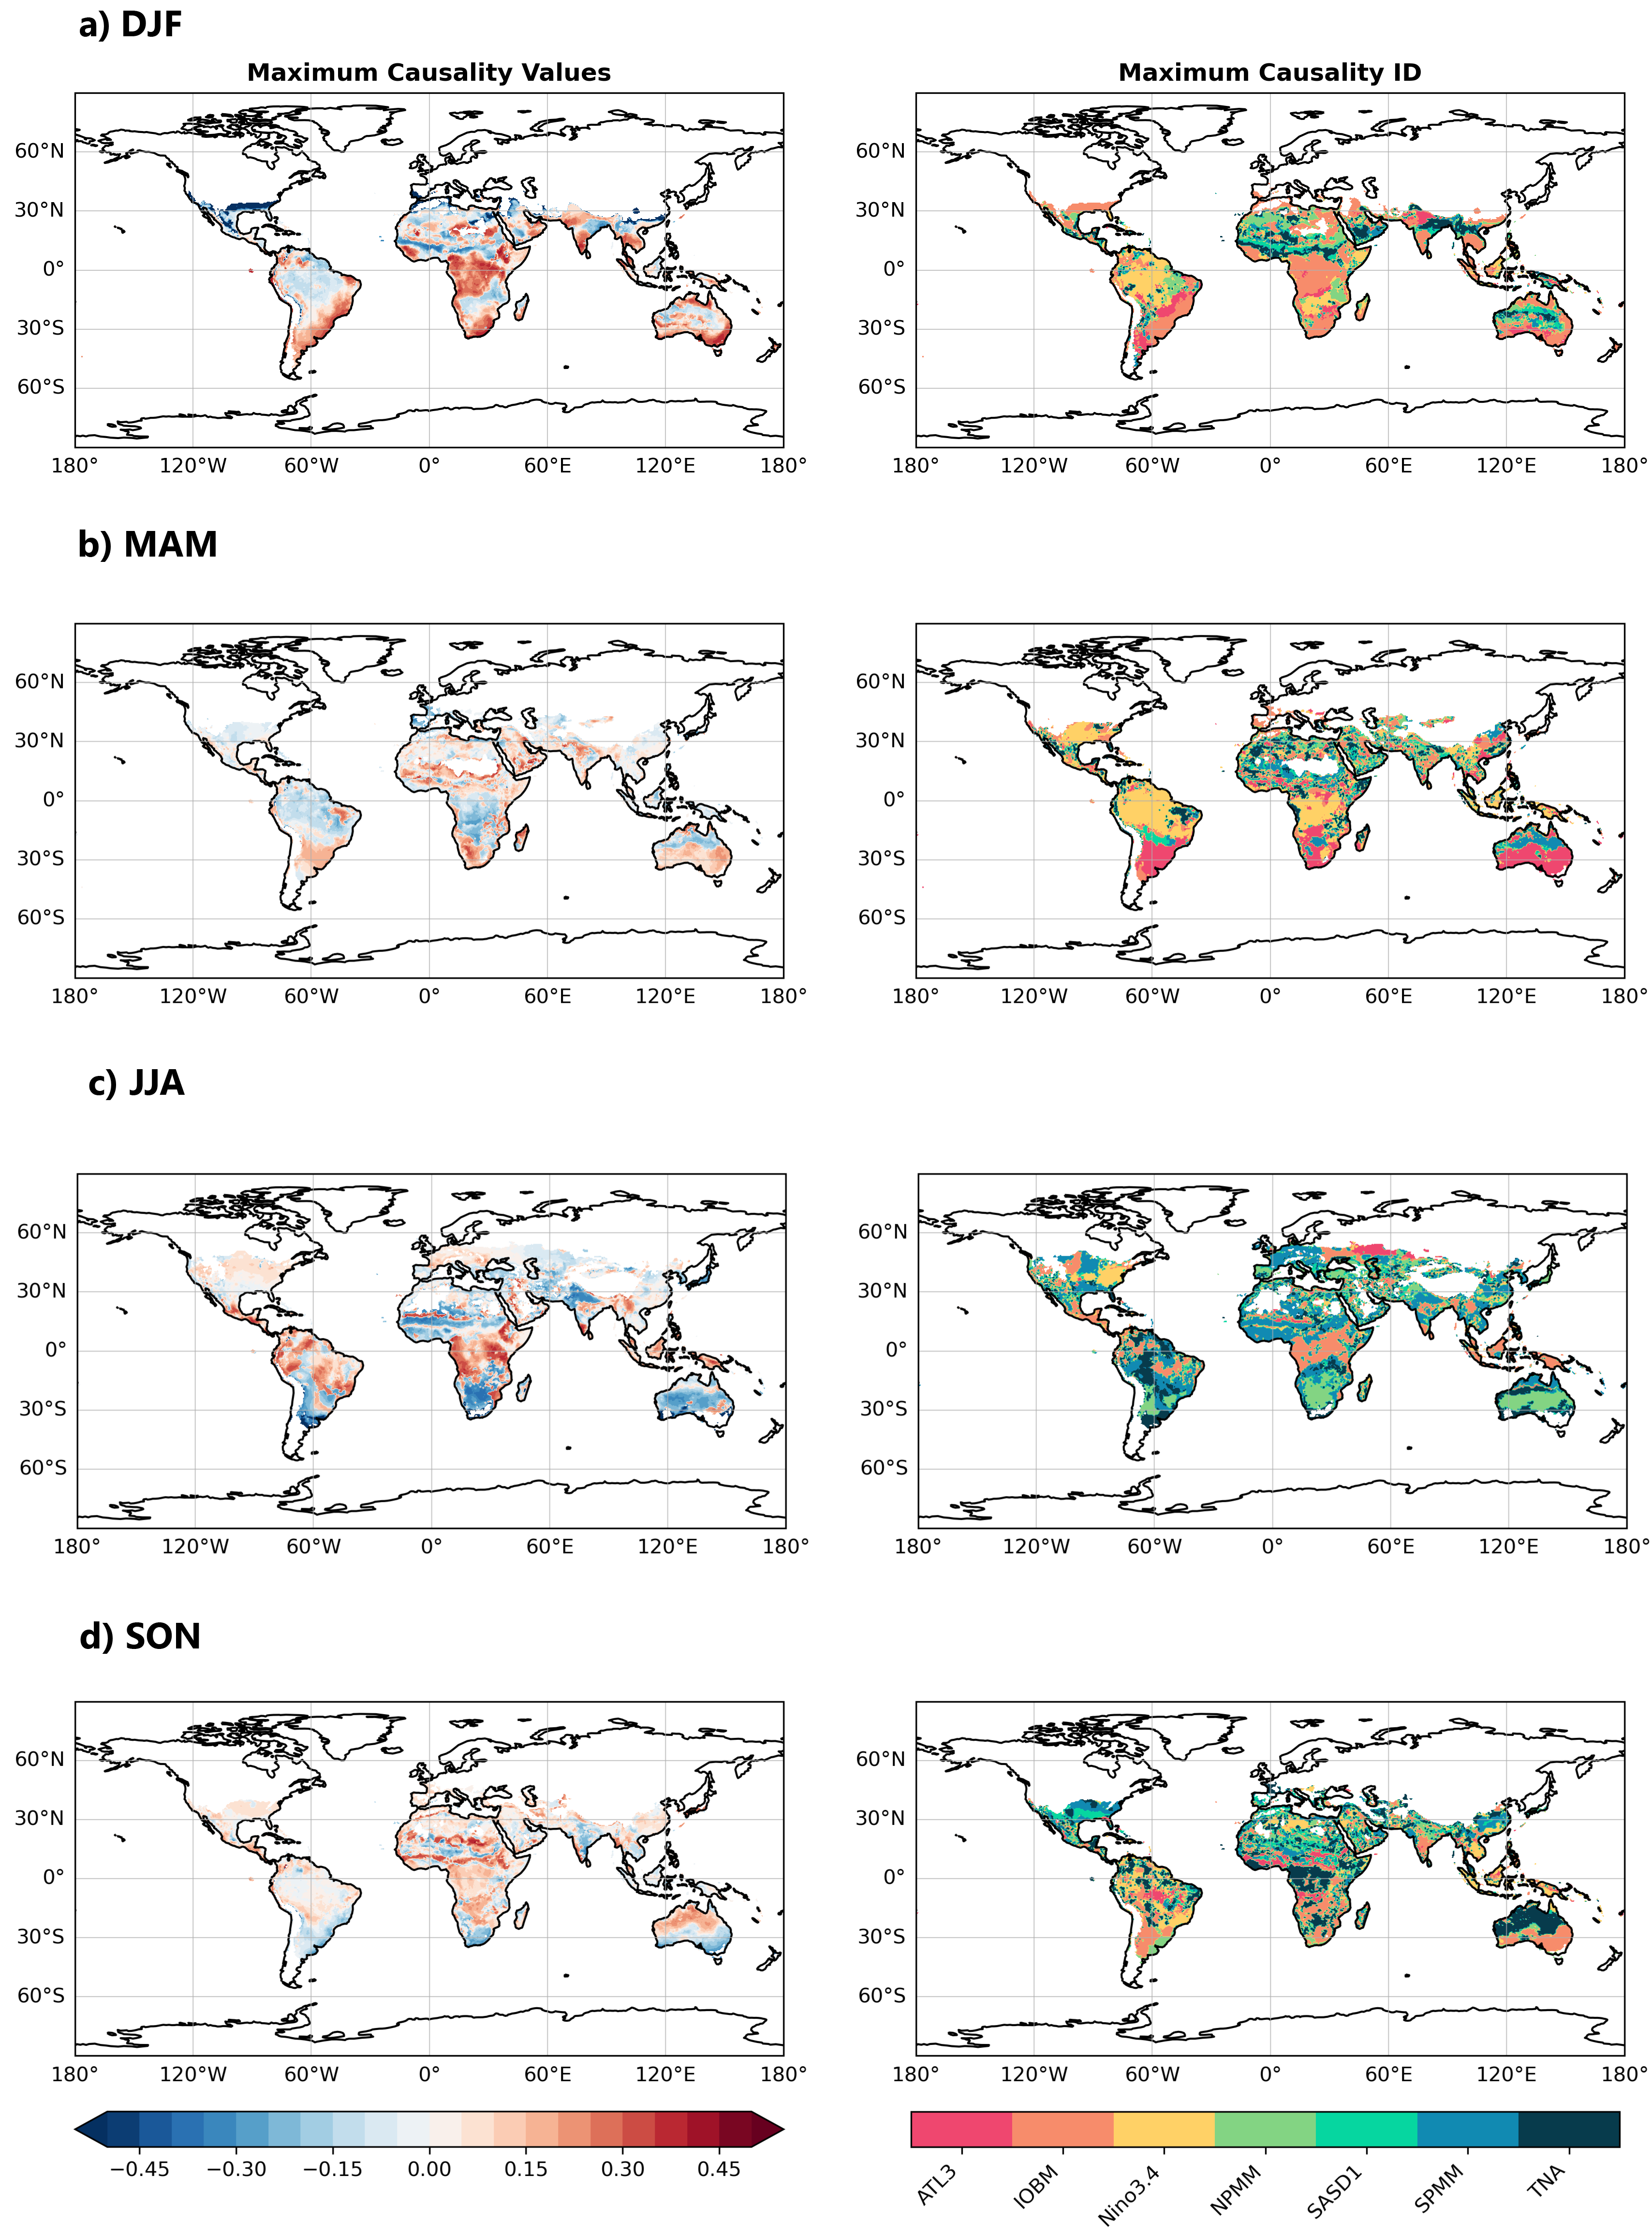
\includegraphics[width=0.9\textwidth]{causality_final_global_ps.png}
  \caption{\textbf{a)-d)} For all seasons: Left, maximum statistically significant causality values between $R_0$ and all indexes of Table \ref{tab:climate-variability-indices}, for the 1951-2024 monthly mean period ($p < 0.01$). Right, which index gives the maximum statistically significant causality values. }
  \label{fig:global-causality-final}
\end{figure*}

\begin{figure*}[!ht]
  \centering
  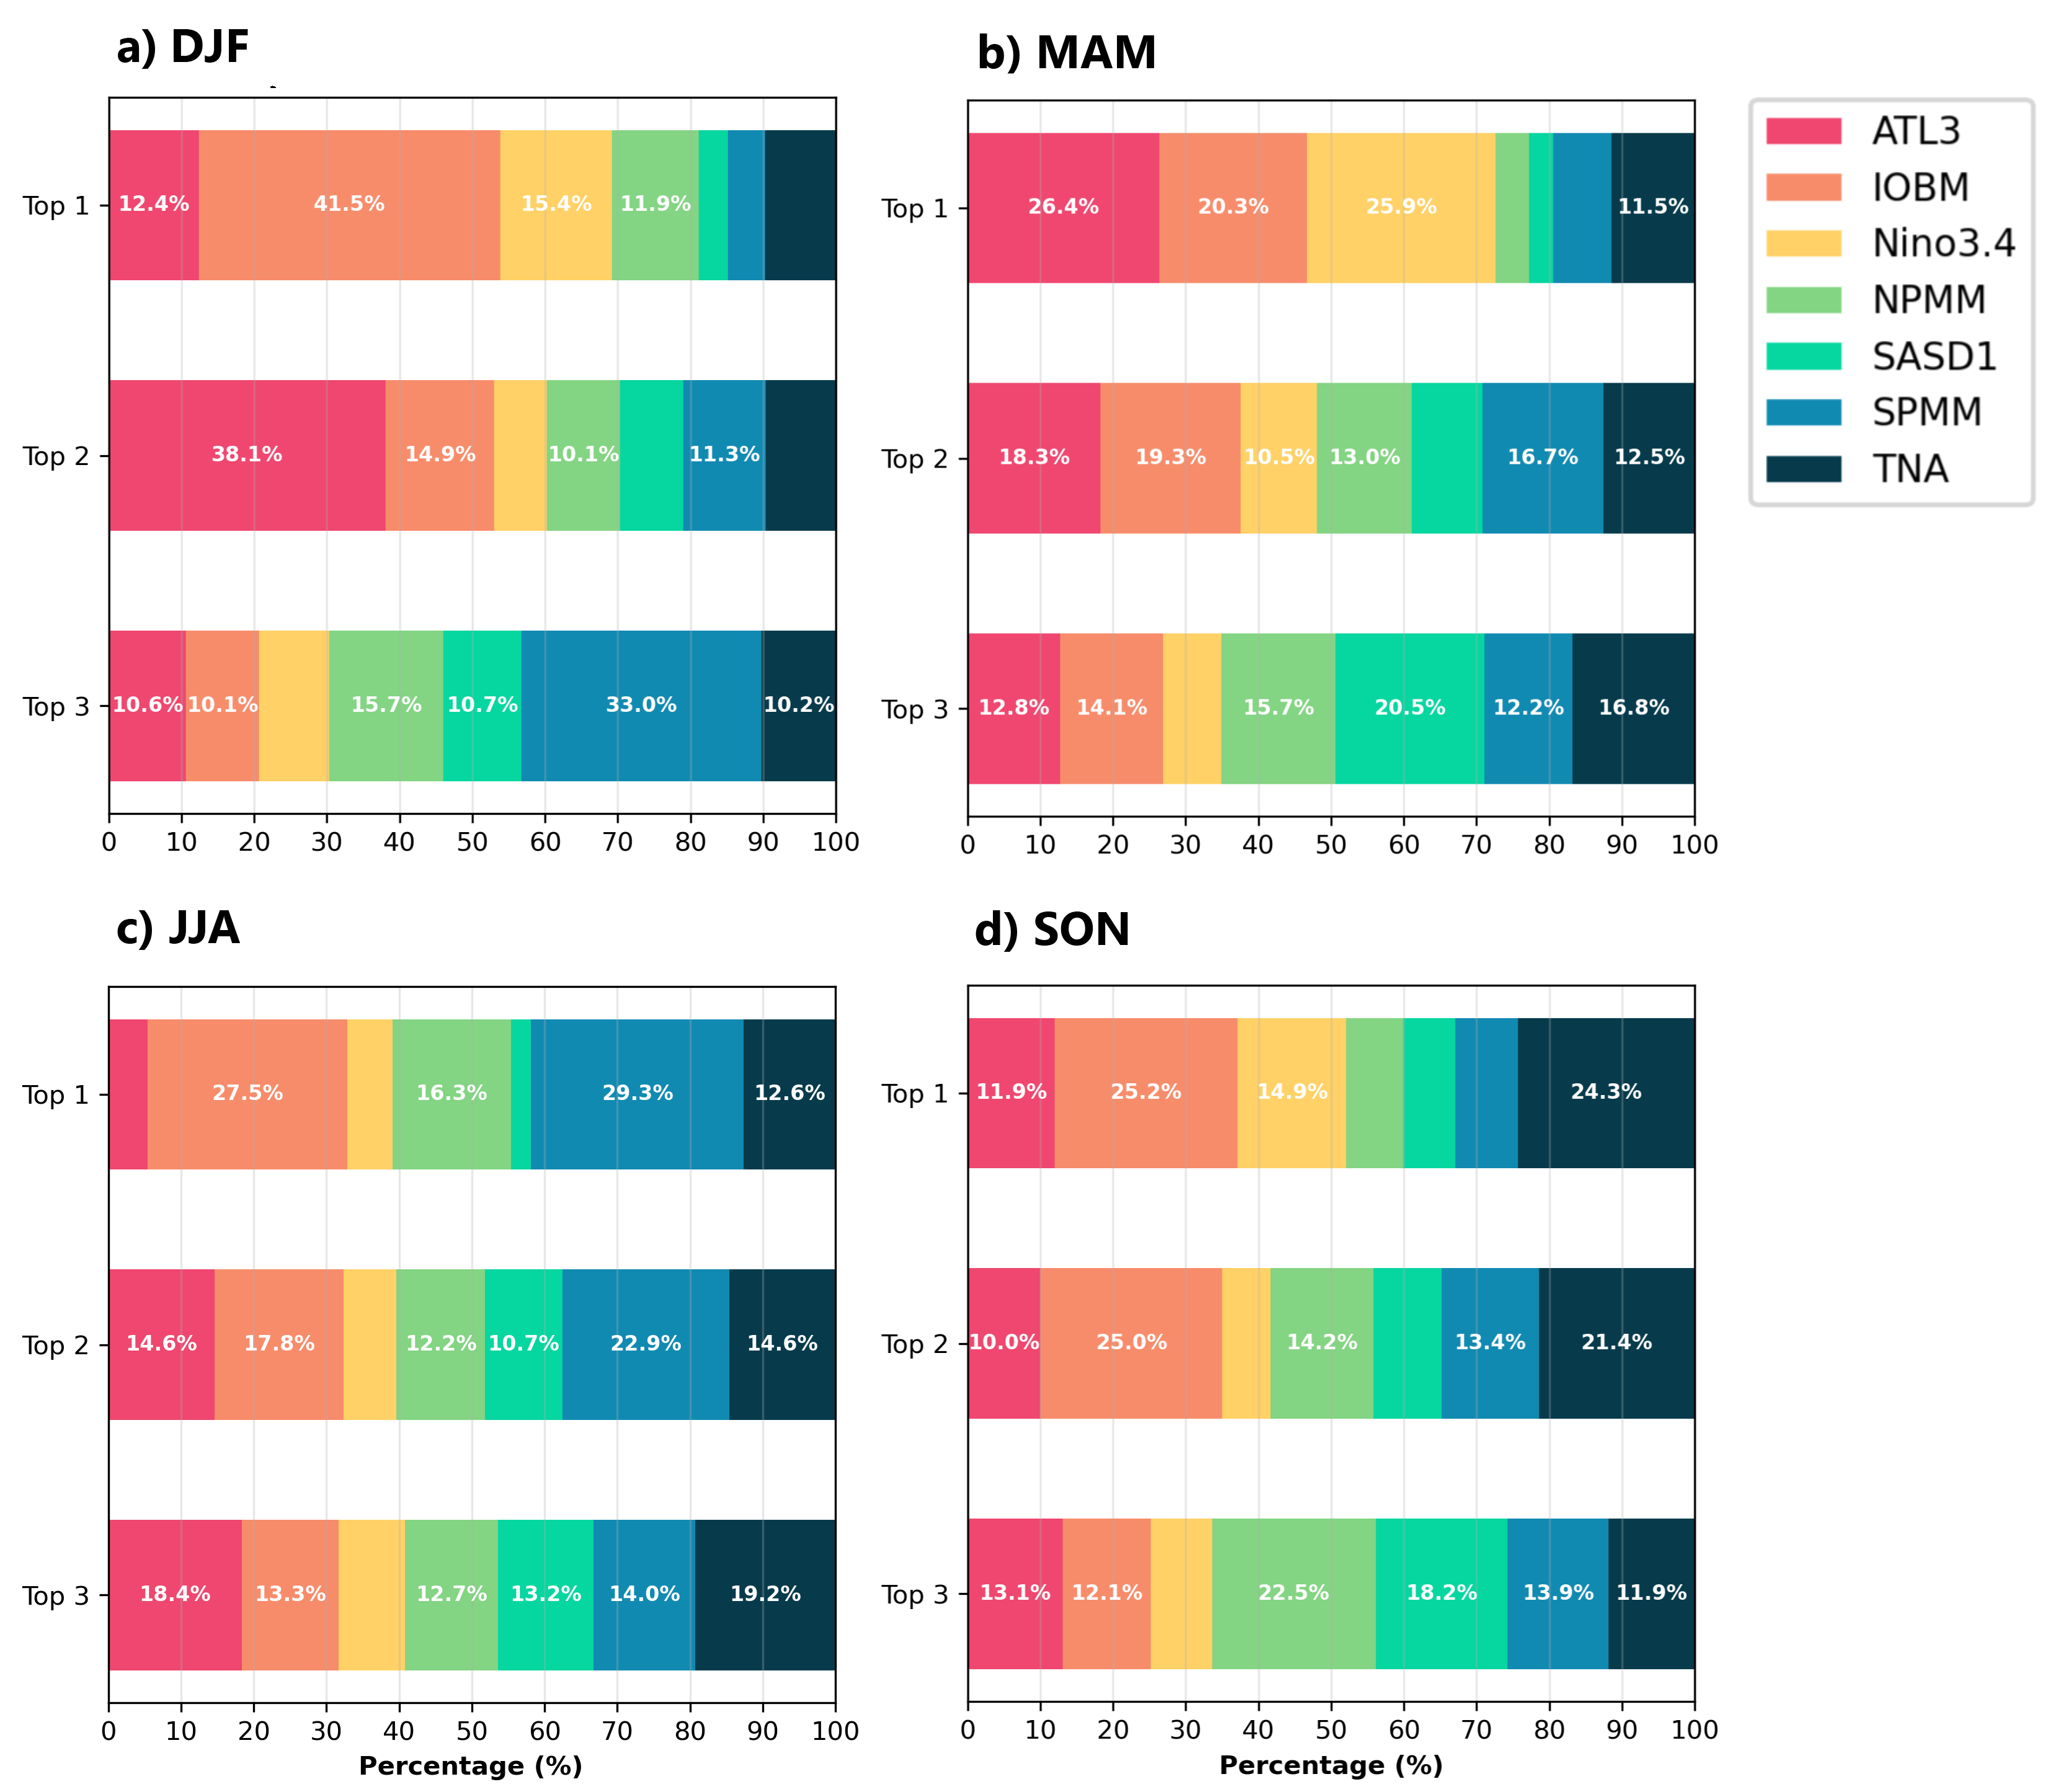
\includegraphics[width=0.75\textwidth]{causality_barplots.png}
  \caption{\textbf{a)-d)} For all seasons: Percentage of grid points over which each index gives the highest, second or third highest statistically significant causality values. Any contribution above 10\% is labeled in the barplots.}
  \label{fig:causality-barplots}
\end{figure*}
\noindent
\\
Over the austral winter (Figure \ref{fig:global-correlation-niño-34}c), the correlation patterns shift overall in the Southern Hemisphere. Fewer regions, with Africa in particular, show predominantly weaker correlation values. Negative correlations additionally emerge over the Sahel region, India and the East Coast of the United States. The austral spring (Figure \ref{fig:global-correlation-niño-34}d) demonstrates a return to stronger correlation patterns, particularly in South America where positive correlations re-intensify across the Amazon and southern Brazil regions.
\\
\\
An aggregate of the maximum statistically significant correlation values between $R_0$ and all climate variability indices, as well as the index that gives the maximum correlation value, is shown in Figure \ref{fig:global-correlation-final}. The left column shows the maximum correlation values for each index, while the right column shows which index gives the maximum correlation value for each grid point. The percentage of grid points over which each index gives the highest statistically significant correlation values is shown in Figure \ref{fig:barplots-correlation}. It is worth noting that, since the difference between correlation values can often be small, the second and third highest correlation values are also shown in the figure, in order to provide a more complete picture of the relative importance of each index.
\\
\\
Over the austral summer and autumn months (Figure \ref{fig:global-correlation-final}a-b) the Niño3.4 index is the most dominant index in the regions previously highlighted in Figure \ref{fig:global-correlation-niño-34}a-b. However, as the Niño3.4 correlation with $R_0$ weakens during the austral winter and spring months over its zones of influence (Figure \ref{fig:global-correlation-niño-34}c-d), other climate indices are vying for dominance in its stead (Figure \ref{fig:global-correlation-final}c-d, right). This behavior is also replicated in the regions of more seasonal $R_0$ variance described in section \ref{sec-results-1}, where the spread of the indices over which maximum correlation is attributed to becomes more heterogeneous (Figure \ref{fig:global-correlation-final}a-d, right). Notable areas include the Sahel region, Mediterranean basin, parts of southern Africa, Australia, the East Coast of the United States and southeastern Asia, where different indices dominate the correlation landscape depending on the season.
\\
\\
With this, it is evident that multiple seasonal temperature-based climate indices compete for dominance across different regions and seasons, with no single index controlling more than 25\% of grid points as the primary correlate, in accordance to Figure \ref{fig:barplots-correlation}. Still, other notable indices include the IOBM index, contributing more than 10\% of grid points in nearly all categories and being prevalent in India during the austral winter and spring months. These findings and results for both El Niño and IOBM are consistent with previous studies that have highlighted the importance of both ENSO and the Indian Ocean in influencing climate variability and its potential impact on \textit{Aedes}-borne disease transmission\cite{chen_2024,kurnianingsih_2020, banu_2015}.
\\
\\
Despite their respective contributions however, the spread of all seven indices is relatively even, with no single index clearly dictating whether $R_0$ is directly tied to one specific climate pattern, reflecting the multifaceted nature of climate variability influence on \textit{Aedes}-borne disease transmission.

\subsection{Analysis 3: Causality studies between $R_0$ and climate variability indices. Outlining of predictors for disease outbreaks} \label{sec-results-3}

Analogues of figures \ref{fig:global-correlation-final} and \ref{fig:barplots-correlation} for section \ref{sec-results-3} are shown in Figures \ref{fig:global-causality-final} and \ref{fig:causality-barplots} for the Liang-Kleeman causality analysis. The causality analysis is performed over the same 1951-2024 monthly mean period, with the same climate variability indices of Table \ref{tab:climate-variability-indices}.
\\
\\
As opposed to the correlation outputs in Figure \ref{fig:global-correlation-final}, the causality analyses in Figure \ref{fig:global-causality-final} show a pronounced attenuation across all different regions and seasons, with the maximum causality values rarely exceeding values over $\pm0.25$. Since causality is a more stringent condition than correlation, as it requires a direct influence of one variable over another, more diffuse and weaker patterns suggest that the direct causal influence of these climate patterns on transmission potential is considerably more modest than simple correlation analysis would suggest. Additionally, since patterns are more spatially fragmented overall, direct causal climate influences on $R_0$ seem to operate through more localized mechanisms, instead of the more broader-scale patterns that correlation analyses might imply.
\\
\\
Nonetheless, the causality analysis still provides valuable insights into the relationships between $R_0$ and climate variability indices. Positive Liang-Kleeman causality indicates that variations in any given climate pattern tend to amplify or destabilize fluctuations over $R_0$ (either favorably or unfavorably), leading to large changes in transmission potential. Alternatively, negative causality values suggest that variations in the climate index tend to dampen or stabilize fluctuations over $R_0$, acting as a regulator for disease transmission and bringing $R_0$ toward more moderate values.
\\
\\
In this context, similarly to the correlation analyses, both the Niño3.4 index and IOBM index are the most dominant causal indices over the austral summer and autumn months over the Amazon basin, central Africa and southeastern regions of Asia (Figure \ref{fig:global-causality-final}a-b), with other indices gaining prominence in these regions during the austral winter and spring months (Figure \ref{fig:global-causality-final}c-d). Niño3.4 shows negative causality values over all seasons (causal and stable). Along with the IOBM index showing negative causality values over the spring and autumn months (Figure \ref{fig:global-causality-final}b, d), both of these climate patterns play a buffering effect, preventing extreme deviations on disease transmission values. On the other hand however, the IOBM index shows positive causality values over the summer and winter months (causal but unstable, \ref{fig:global-causality-final}a, c), aligning with the seasonal maximum and minimum of the pattern. It is during these months of peak DENV transmission in both hemispheres that this climate pattern pushes already marginal transmission conditions toward more extreme states: either making cold regions less suitable for transmission, or amplifying transmission windows in suitable or unsuitable areas.
\\
\\
The influence of both Niño3.4 and IOBM indices on $R_0$ is through causality relationships can be seen in Figure \ref{fig:causality-barplots}. While both indices do show a sizable contribution over all categories, similarly to correlation, there is no clear dominance of any index during any season, with the second and third highest causality values being relatively evenly distributed across the different indices. Still, a notable shift occurs during boreal autumn and spring months (\ref{fig:causality-barplots}b, d), with ATL3 gaining increased prominence while maintaining the multi-index influence pattern. The NPMM and SASD1 indices maintain substantial influence, while other indices show varying degrees of contribution. All of these ocean-based patterns show varying degrees of influence across regions with high seasonality (\ref{fig:global-causality-final}b, d), suggesting that ocean basins become drivers of transmission variability at different times of the year in these areas.

\section{Discussion} \label{sec-discussion}

\subsection{The added value of climate patterns in seasonal forecasting of \textit{Aedes}-borne diseases} \label{sec-discussion-added-value}

\subsection{Analysis 1: Multi-timescale climate decomposition of $R_0$} \label{sec-discussion-analysis-1}

\subsection{Analyses 2 and 3: Correlation and causality studies between $R_0$ and climate variability indices} \label{sec-discussion-analysis-2-3}

\subsection{Notable constraints and limitations} \label{sec-discussion-limitations}

A number of caveats should be acknowledged when interpreting the results of this study or translating these findings into public health applications.
\\
\\
It is known that \textit{Aedes}-borne diseases are not only driven by climate, but also by mosquito presence in any affected hotspot, as well as socio-economic factors such as population density, urbanization, and public health infrastructure, as previously explained in Section \ref{sec-methods-redefining-R0}. As such, while the results of this study, which are constrained to the climate-driven component of disease transmission, are indeed valuable, it needs to be emphasized that the interplay between these factors is complex and context-dependent, and that climate, while crucial, is just one piece of the puzzle. In the context of the creation of a climate-driven DENV forecasting system using these results, health officials must take into account the multi-faceted nature of these drivers (mosquito presence, socio-economic factors, climate conditions) in order for disease control programs to be more effective.
\\
\\
Second, it is of note that while the results that were presented throughout this manuscript cover a wide temporal range, the analysis is still based on global datasets. As such, the applicability of these findings to specific DENV hotspots should be carefully considered, with the use of high-resolution observational data being encouraged to reproduce and build on these results in a local context.
\\
\\
Additionally, while these findings have been obtained with careful data handling in avoiding edge cases, correlation and causality analyses in regions where data is spurious or where the $R_0$ signal is weak (i.e., in temperate regions with low transmission potential) may not yield reliable or realistic results. Computation for both analyses are reliant on the variance or covariance of the data available, and therefore, where there are few data points, these statistics become unstable and sensitive, leading to artificially large or small values.
\\
\\
Lastly, it is worth commenting that the choice of climate patterns in Table \ref{tab:climate-variability-indices} is not exhaustive. While the seven climate patterns that were selected do share similarities with one another (temperature-based seasonal patterns, with some of them being precursors of El Niño), other relevant seasonal patterns have been omitted from the analysis. Including more climate patterns is out of the scope of this study, though we encourage future studies to expand on the results presented here.

\section{Conclusions} \label{sec-conclusions}

\begin{enumerate}
  \item Historical reconstructions of climate-driven $R_0$ values for \textit{Aedes}-borne diseases provide valuable insight in the role of climate in disease emergence, and can be used to improve the accuracy of seasonal DENV forecasts through the identification of predictors in the form of broad-scale climate patterns.
  \item Long-term, man-made climate change is shown to have a significant impact on the environmental suitability for \textit{Aedes}-borne diseases in the tropics, which comprise the Amazon basin, central Africa, and Southeast Asia. As the effects of climate change intensify, bordering regions that shift into A-type climate zones in the Köppen-Geiger classification may experience potential shifts in transmission patterns.
  \item Whereas tropical regions show a more stable but high $R_0$ signal throughout the year, temperate regions exhibit a pronounced seasonal component, with peak transmission values occurring during the summer months. The difference in $R_0$ climatology plays a crucial role in the development of DENV early warning systems and allocation of resources for vector and disease control.
  \item Correlation and causality analyses are complimentary concepts that can be used to understand the role of climate patterns in the dynamics of \textit{Aedes}-borne diseases. While correlation exemplifies the strength and direction of relationships between variables, causality corroborates or refutes these relationships, while also providing insight into its stability.
  \item ENSO and IOBM are shown to be the most dominant climate patterns in regions where the long-term climate signal is stronger (Amazon basin, central Africa and southeastern Asia). However, other temperature-based seasonal patterns gain prominence during the austral winter and spring months, especially over regions with a stronger seasonal transmission component. Overall, no single climate pattern dominates the transmission landscape; it is the compound effects of multiple patterns that ultimately shape the dynamics of DENV outbreaks, and their combined influence should be considered in the development of \text{Aedes}-borne disease prediction systems.
  \item In the tropics, periods of El Niño act as a promoter of \textit{Aedes}-borne disease transmission, while periods of La Niña serve as a suppressor. Regardless of the phase however, ENSO is a stabilizing factor for DENV outbreaks in the tropics, preventing extreme deviations and keeping transmission potential high. IOBM shows similar behavior, though during peak DENV transmission months, it can push marginal transmission conditions toward more extreme states, making cold regions less suitable for transmission, or warming suitable or unsuitable areas to amplify transmission windows.
  \item While global climate patterns are suitable for a broad, general-purpose understanding, high-resolution data is preferred when analyses are performed in endemic regions or hotspots, in order to account for more nuanced local-scale phenomena and provide more accurate and actionable information for public health officials.
\end{enumerate}

\noindent Given the above, future work should focus on the integration of high-resolution climate data and local-scale factors into seasonal DENV forecasting models. A framework for the development of such a model is currently being developed, to be reported in future publications.

\section*{Additional files} \label{sec-additional-files}

\href{multilingual_abstracts.pdf}{Additional file 1}: Multilingual abstracts in the six official working languages of the United Nations.

\section*{Abbreviations} \label{sec-abbreviations}
AeDES2: \textit{Ae}des \textit{D}isease \textit{E}nvironmental \textit{S}uitability 2; AIC: Akaike Information Criterion; ATL3: Atlantic 3 Index; CHIKV: Chikungunya; DENV: Dengue; ENSO: El Niño Southern Oscillation; GCV: Generalized cross-validation; IOBM: Indian Ocean Basin; LOESS: Locally estimated scatterplot smoothing; NPMM: North Pacific Meridional Mode; $R^2$: Coefficient of determination; SASD: South Atlantic Subtropical Dipole; SPMM: South Pacific Meridional Mode; TNA: Tropical North Atlantic; VBDs: Vector-borne diseases; WHO: World Health Organization; ZIKV: Zika.

\section*{Acknowledgements} \label{sec-acknowledgements}

(Blank until we figure coauthor contributions)

\section*{Funding} \label{sec-funding}

(Same here, blank for now)

\section*{Availability of data and materials} \label{sec-availability}
Code for the generation of $R_0$ values employed for this study, computed using AeDES2's monitoring system, is available under request for any region and grid-point. Additionally, the necessary datasets, functions and scripts to generate the maps and plots for this manuscript and supplementary material are available under the following GitHub repository: \url{https://github.com/jacorvillo/monitoring_system_analysis}

\section*{Authors' contributions} \label{sec-authors-contributions}

Á.M., V.T. and D.C. conceived the methodology to be undertaken in this manuscript. Data sources, code and figures were obtained and developed from the ground up by J.C, who also analysed the results. All authors have reviewed the manuscript.

\section*{Ethics approval and consent to participate} \label{sec-ethics-approval}
Not applicable.

\section*{Consent for publication} \label{sec-consent-for-publication}
Not applicable.

\section*{Competing interests} \label{sec-competing-interests}
The authors declare no competing interests.

\bibliography{references}

\end{document}